
\documentclass[a4paper]{article}

%% Language and font encodings
\usepackage[english,spanish]{babel}
\usepackage[utf8x]{inputenc}
\usepackage[T1]{fontenc}

\usepackage{lipsum}

%\bibliographystyle{apalike} %% Sets page size and margins
\usepackage[round]{natbib}
\bibliographystyle{plainnat}
%\usepackage[a4paper,top=3cm,bottom=2cm,left=3cm,right=3cm,marginparwidth=1.75cm]{geometry}

%% Useful packages
\usepackage{amsmath}
\usepackage{graphicx}
\usepackage[colorinlistoftodos]{todonotes}
\usepackage[colorlinks=true, allcolors=blue]{hyperref}
\usepackage{subfigure} 
\usepackage{float}
\usepackage{verbatim}
\usepackage{appendix}

\addtolength{\subfigcapskip}{-10pt}
\addtolength{\subfigbottomskip}{-30pt}
%\addtolength{\subfigcapmargin}{-30pt}


%\addtolength{\subfigtopskip}{-25pt}

\graphicspath{{../plots/}}

\usepackage{listings}
\usepackage{xcolor}


\lstset{language=R,
	basicstyle=\small\ttfamily,
	stringstyle=\color{DarkGreen},
	otherkeywords={0,1,2,3,4,5,6,7,8,9},
	morekeywords={TRUE,FALSE},
	deletekeywords={data,frame,length,as,character},
	keywordstyle=\color{blue},
	commentstyle=\color{DarkGreen},
}



\renewenvironment{abstract}{
	\vspace*{\fill}
	\begin{center}%
		\bfseries\abstractname
\end{center}}%
{\vfill}


%% authors
\usepackage{authblk}
\title{Old series, new signals \\
	 {\large The economic cycle in light of wavelet analysis} }
\author[1]{Diego Kozlowski}
\affil[1]{Master in Data Mining \& Knowledge Discovery, FCEN-UBA \\ diegokoz92@gmail.com}

\date{}                     %% if you don't need date to appear
\setcounter{Maxaffil}{0}
\renewcommand\Affilfont{\itshape\small}


\begin{document}


\maketitle


\selectlanguage{english}
	\begin{abstract}
	The economic cycle is a subject of recurring debate in the specialized bibliography. Both from the conceptual point of view and its empirical recognition, there is no general consensus regarding the causes and concrete forms of this characteristic of the economy. In particular, the statements regarding the existence of a long wave, proposed by different authors of the early twentieth century, are a source of debate. In this work we propose an empirical review of series traditionally used in economic analysis, such as the product, wages and gold, for the United States and the United Kingdom, from the 18th century to the present, using a technique originally developed in the area of ​​signal analysis. The objective is to seek new evidence regarding the presence of a well-defined cycle in long periods of economic history. For this, the Wavelets analysis is used in search of low frequency signals, or long periods. The results show favorable evidence to the existence of three well-defined cycles, one of which would be of an amplitude around 50 years.
	\end{abstract}

\selectlanguage{spanish}	
	\begin{abstract}
		El desenvolvimiento cíclico de la economía es un tema de recurrente debate en la bibliografía especializada. Tanto desde el punto de vista conceptual como en el reconocimiento empírico, no existe un consenso generalizado respecto de las causas y formas concretas de esta característica de la economía. En particular, son fuente de debate las afirmaciones respecto a la existencia de ciclos definidos en períodos largos, propuestos por diferentes autores de principios del siglo XX. En el presente trabajo se propone una revisión empírica de series tradicionalmente utilizadas en el análisis económico, como lo son el producto, salario y oro, para Estados Unidos y el Reino Unido, desde el siglo XVIII a la actualidad, mediante una técnica originalmente desarrollada para el área de análisis de señales. El objetivo es buscar nuevas evidencias respecto a la presencia de un ciclo bien definido en períodos largos de la historia económica. Para esto, se utiliza el análisis de Wavelets en busca de señales de baja frecuencia, o períodos largos. Los resultados muestran evidencia favorable a la existencia de tres ciclos bien definidos, uno de los cuales sería de una amplitud en torno a los 50 años.
	\end{abstract}

\selectlanguage{english}

\section{Introduction}
 
In economic theory there is no unequivocal position regarding the cyclical forms of economic development. The long waves proposed by \cite{kondratieff1979long} of approximately 50 years span and the medium waves proposed by \cite{kuznets1930secular} have result in controversy throughout the 20th century. To a large extent this debate is due to the fact that there is no unambiguous expression of what is called \textit{economic development}. In the first place, it doesn't exist a single variable that captures this concept as a hole, but it can only be represented fragmentarily in variables such as the Gross Domestic Product (GDP), the Wages, or the Interest Rate. But even if we could have a single variable that completely measures the economic development, the national delimitation of the measurements is still remaining. The latter comes from the fact that what is considered as the economic cycle refers to a fundamental characteristic of the economic system, which is not necessarily mediated by national divisions. That is to say, it is a phenomenon proper to capitalism as a system, and does not necessarily reproduce itself fully within each country.


These complexities for measuring the economic cycle make it difficult to understand it. The goal of this paper is to make use of new quantitative tools for the analysis of time series, to review the empirical evidence regarding the existence of the economic cycle. Given the limitations mentioned above, it was decided to use series from the United States because it is a country that due to its size achieves, from the 20th century, to represent, at least partially, the general tendencies of the economy. For methodological reasons, it is necessary that the information used goes back to the 19th century, a century in which it is not clear that the general characteristics of economic development are expressed within this country. That is why for the eighteenth and nineteenth centuries the study is complemented with the product series for the United Kingdom.

The paper is structured as follows: After this introduction, a summary of the main debates regarding the economic cycle that took place during the 20th century is presented. In the third section an exploratory data analysis is carried out, where the different series used in the rest of the work are observed, as well as the characteristics of the gold price series and its effects on the rest of the data. Finally some of the series along with the known crises in the economic historiography for the United States in the 20th century are presented. The fourth section proposes the use of the wavelet technique to model the economic cycle and we observe the results of applying this methodology to the GDP and wages series. Finally, the fifth and final section presents the conclusions and future lines of work.


\section{Debates around the economic cycle}

There are not many polemics in the economic literature in which position has been taken from practically all the schools of economic thought. The discussion around what is the economic cycle? How does it originate? And what implications does it have at the level of economic policy, is for sure one of those controversies.

From all schools of economic thought it have been sought explanations to these questions. On the one hand, we find the explanations that focus on the role of demand, particularly investment goods, as the starting point of the economic cycle. There, in the work of \cite{kalecki2013essays} the cycle arises by the particular dynamics of the demand for investment goods from the temporary differences between the decisions of demand for these goods and the moment when they are finally set in motion. Then \cite{keynes2018general} argues that \textit{animal spirits} dominate the scene, with the marginal efficiency of capital guiding the cycle path. Also belong to this school \cite {harrod1936trade}, \cite{kaldor1940model} and \cite{samuelson1939synthesis}, who propose models where there is an interaction between the Keynesian multiplier and the acceleration principle. That is, where the product defines the demand for consumption goods, and this determines the demand for investment goods, which then operate on the product, generating a spiral of over-determinations that end up producing a cycle.

From a different school of thought \cite{schumpeter1939business} begins with the role of innovative entrepreneurs to reach a "tricyclic model" where a superposition of short, medium and long waves operates.
The Austrian theory of the cycle, headed by \cite{hayek1933} and \cite{von1943elastic}, considers a purely monetary origin, based on the endogenous creation of purchasing power and changes in relative prices.

Finally, there is the neoclassical theory of the cycle, which emerges from Lucas's critique of Keynesian macroeconomics. In this kind of models, the microfundation of behavioral assumptions is prioritized. This means that individuals are rational agents, and that at all times there are competitive equilibriums. These models are divided between those proposed by \cite{lucas1975equilibrium} where the initial shock is monetary, and the models of the real business cycle \citep{plosser1989understanding} where the original impulse is given by random changes in technology.

From the point of view of the empirical analysis, there are multiple authors who have found evidence, either through the detailed study of different series \citep{kuznets1930secular, kondratieff1979long, schumpeter1939business}; or using autoregressive models, of moving averages and ARIMA \citep {hamilton1989new, kaiser2012measuring}; or more recently by using wavelets \citep {yogo2008measuring, soares2011business}. Notwithstanding the latter, the use of new empirical techniques for cycle analysis remains a fertile ground for research.

\section{Exploratory Data Analysis}

In the present section we will carry out a brief exploratory analysis of data to observe the general characteristics of the series.

\subsection{Information sources}

Given that the objective of this paper is to perform an analysis of the economic cycle that takes Kondratieff's long waves into consideration, it is necessary to have information as widespread as possible, and therefore use different sources.

For the United States GDP, the data from 1929 to the present comes from the information provided by the \textit{Bureau of Economic Analysis} of that country. For the data from 1790 to 1929 the series elaborated by \cite{johnston2018us} was used.

For the annual series of the nominal hourly wage of production workers in the United States, the information found in \cite{officer2009two} and complemented by \cite{Roesch2018} was used. Nowadays this series corresponds to the item \textit{Employer Costs for Employee Compensation, Total Compensation, Manufacturing, Private Industry} from the series of the \textit{Bureau of Labor Statistics} of the United States.

The annual series of gold prices in the New York market between 1791 and 2017 is based on \cite{officer2018gold}

To analyze the period preceding 1900 the UK GDP series expressed in gold was used. Given the changes in the geopolitical boundaries of the United Kingdom, it was decided to use a series that was consistent intertemporally, the objective being to recognize fluctuations that do not depend on changes in the registration limits. For this, the nominal GDP series between 1700 and 1900 of \cite{Williamson2018uk} was used. The price of gold in the London market for the period 1718-1900 and the official British price for the period 1700-1718 were both recovered from \cite{officer2018gold}


\subsection{Original series}

The figure \ref{fig:oro} shows the value of an ounce of gold in nominal dollars in the New York market, between 1791 and 2017. There, the exit from the gold standard of the world economy is marked in 1971. After the second world war and until that year, the global monetary structure was based on parity with the dollar and the \textit{nominal anchor} of the same with the gold reserves of the Federal Reserve Board (FED). This means that the United States could not issue dollars that were not backed by their gold equivalent in the reserves of the central bank of that country. Therefore, the dollar-gold ratio remained practically unchanged until 1971. After eliminating this anchor, the capacity of free issuance without backup in gold allowed the FED to issue above the reserves it had, and in general, over gold in circulation. This has led to an increase in the price of gold expressed in dollars, or equivalently, a fall in the US dollar expressed in gold.

\begin{figure}[H]
	\centering
	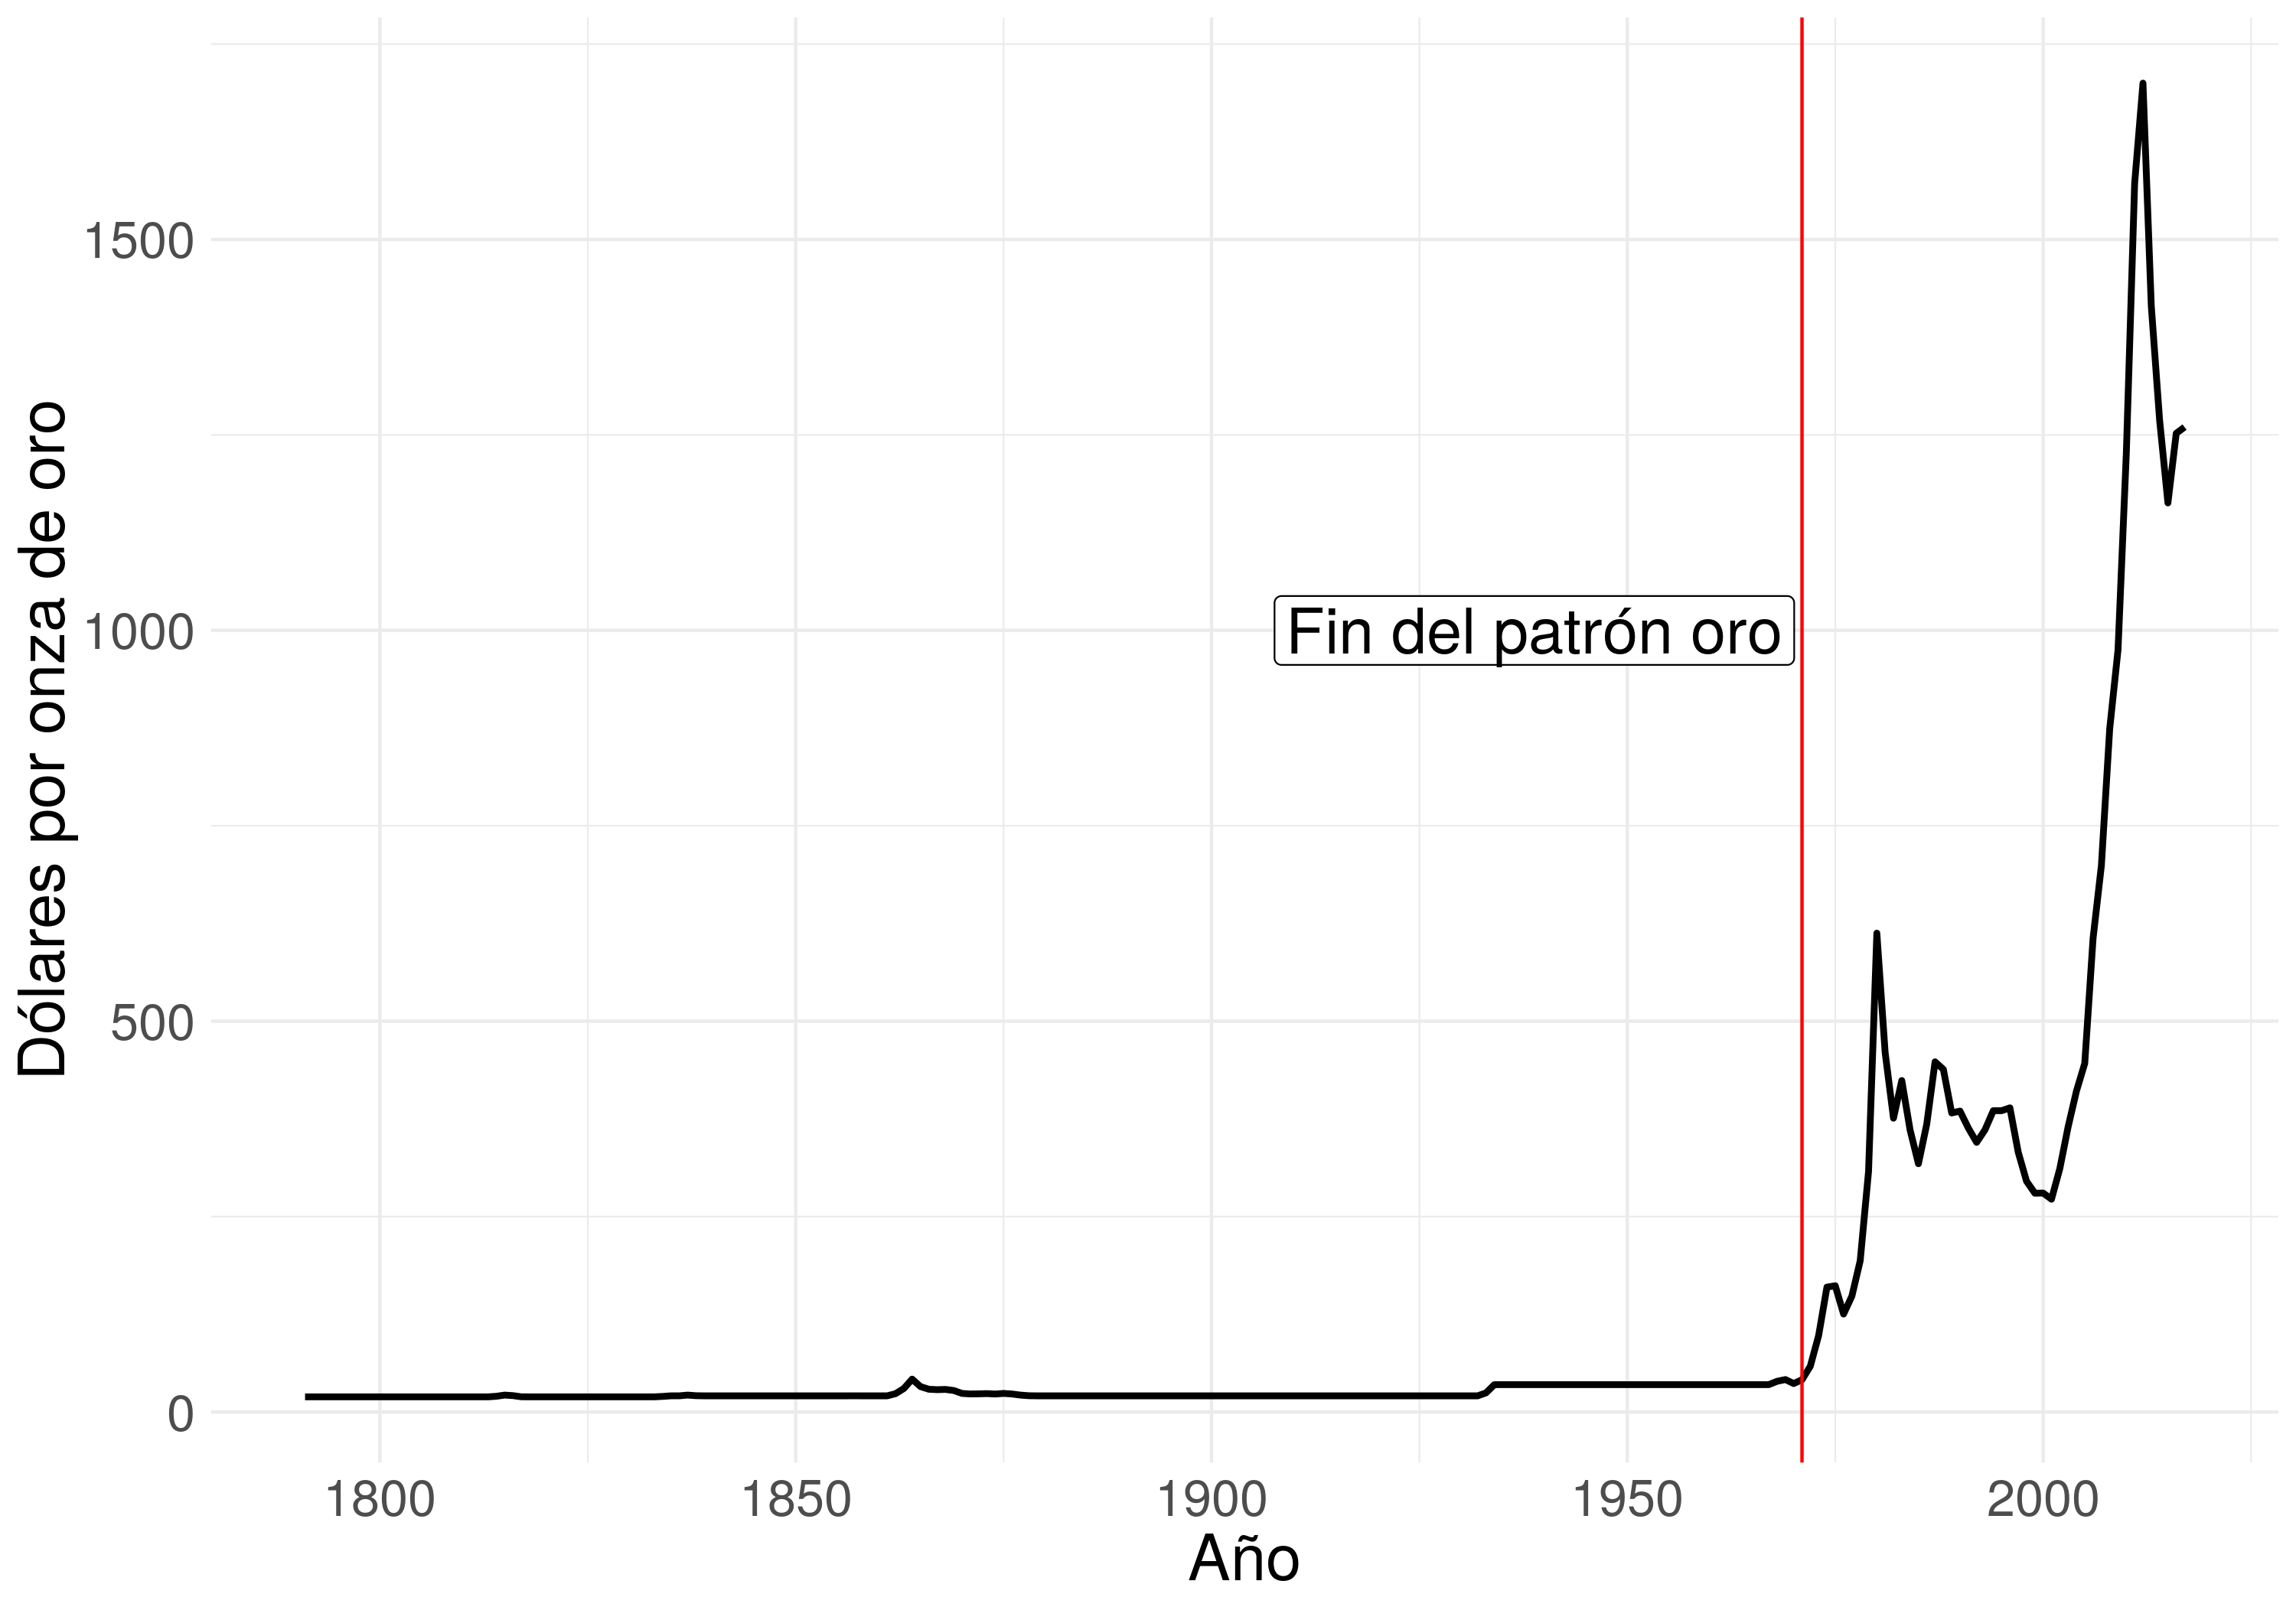
\includegraphics[width=0.75\linewidth]{oro.png}
	 \caption{}\label{fig:oro}
\end{figure}

Given that what is sought in this paper is a long-term analysis of the economic cycle, this nominal disturbance obscures the underlying phenomenon that is being searched. That is why we choose to normalize the nominal GDP series and the nominal wage by the price of gold. In this sense, the series is read as the product and wage expressed in its capacity to purchase gold.


Since gold is a refuge of value in crisis periods, its price is counter-cyclical, a difference from what happens with the Consumer Price Index (CPI). Therefore normalizing by gold instead of CPI gives a better comprehension of the cycle in the series studied and the empirical analysis is facilitated.

According to the above, the figure \ref{fig:PBI} shows the series of the United States GDP between 1900 and 2017, expressed in gold. Meanwhile the figure \ref{fig:salary} shows the series of the hourly wage of a worker of production in the United States between 1900 and 2017, also expressed in gold.

In both cases the periods of economic distress known by the literature are highlighted in red, and in punctuated lines those punctual crises that occurred in a particular year. The table \ref{tabla_crisis} marks the detail of these.


\begin{figure}[H]
	\centering
	\subfigure[]{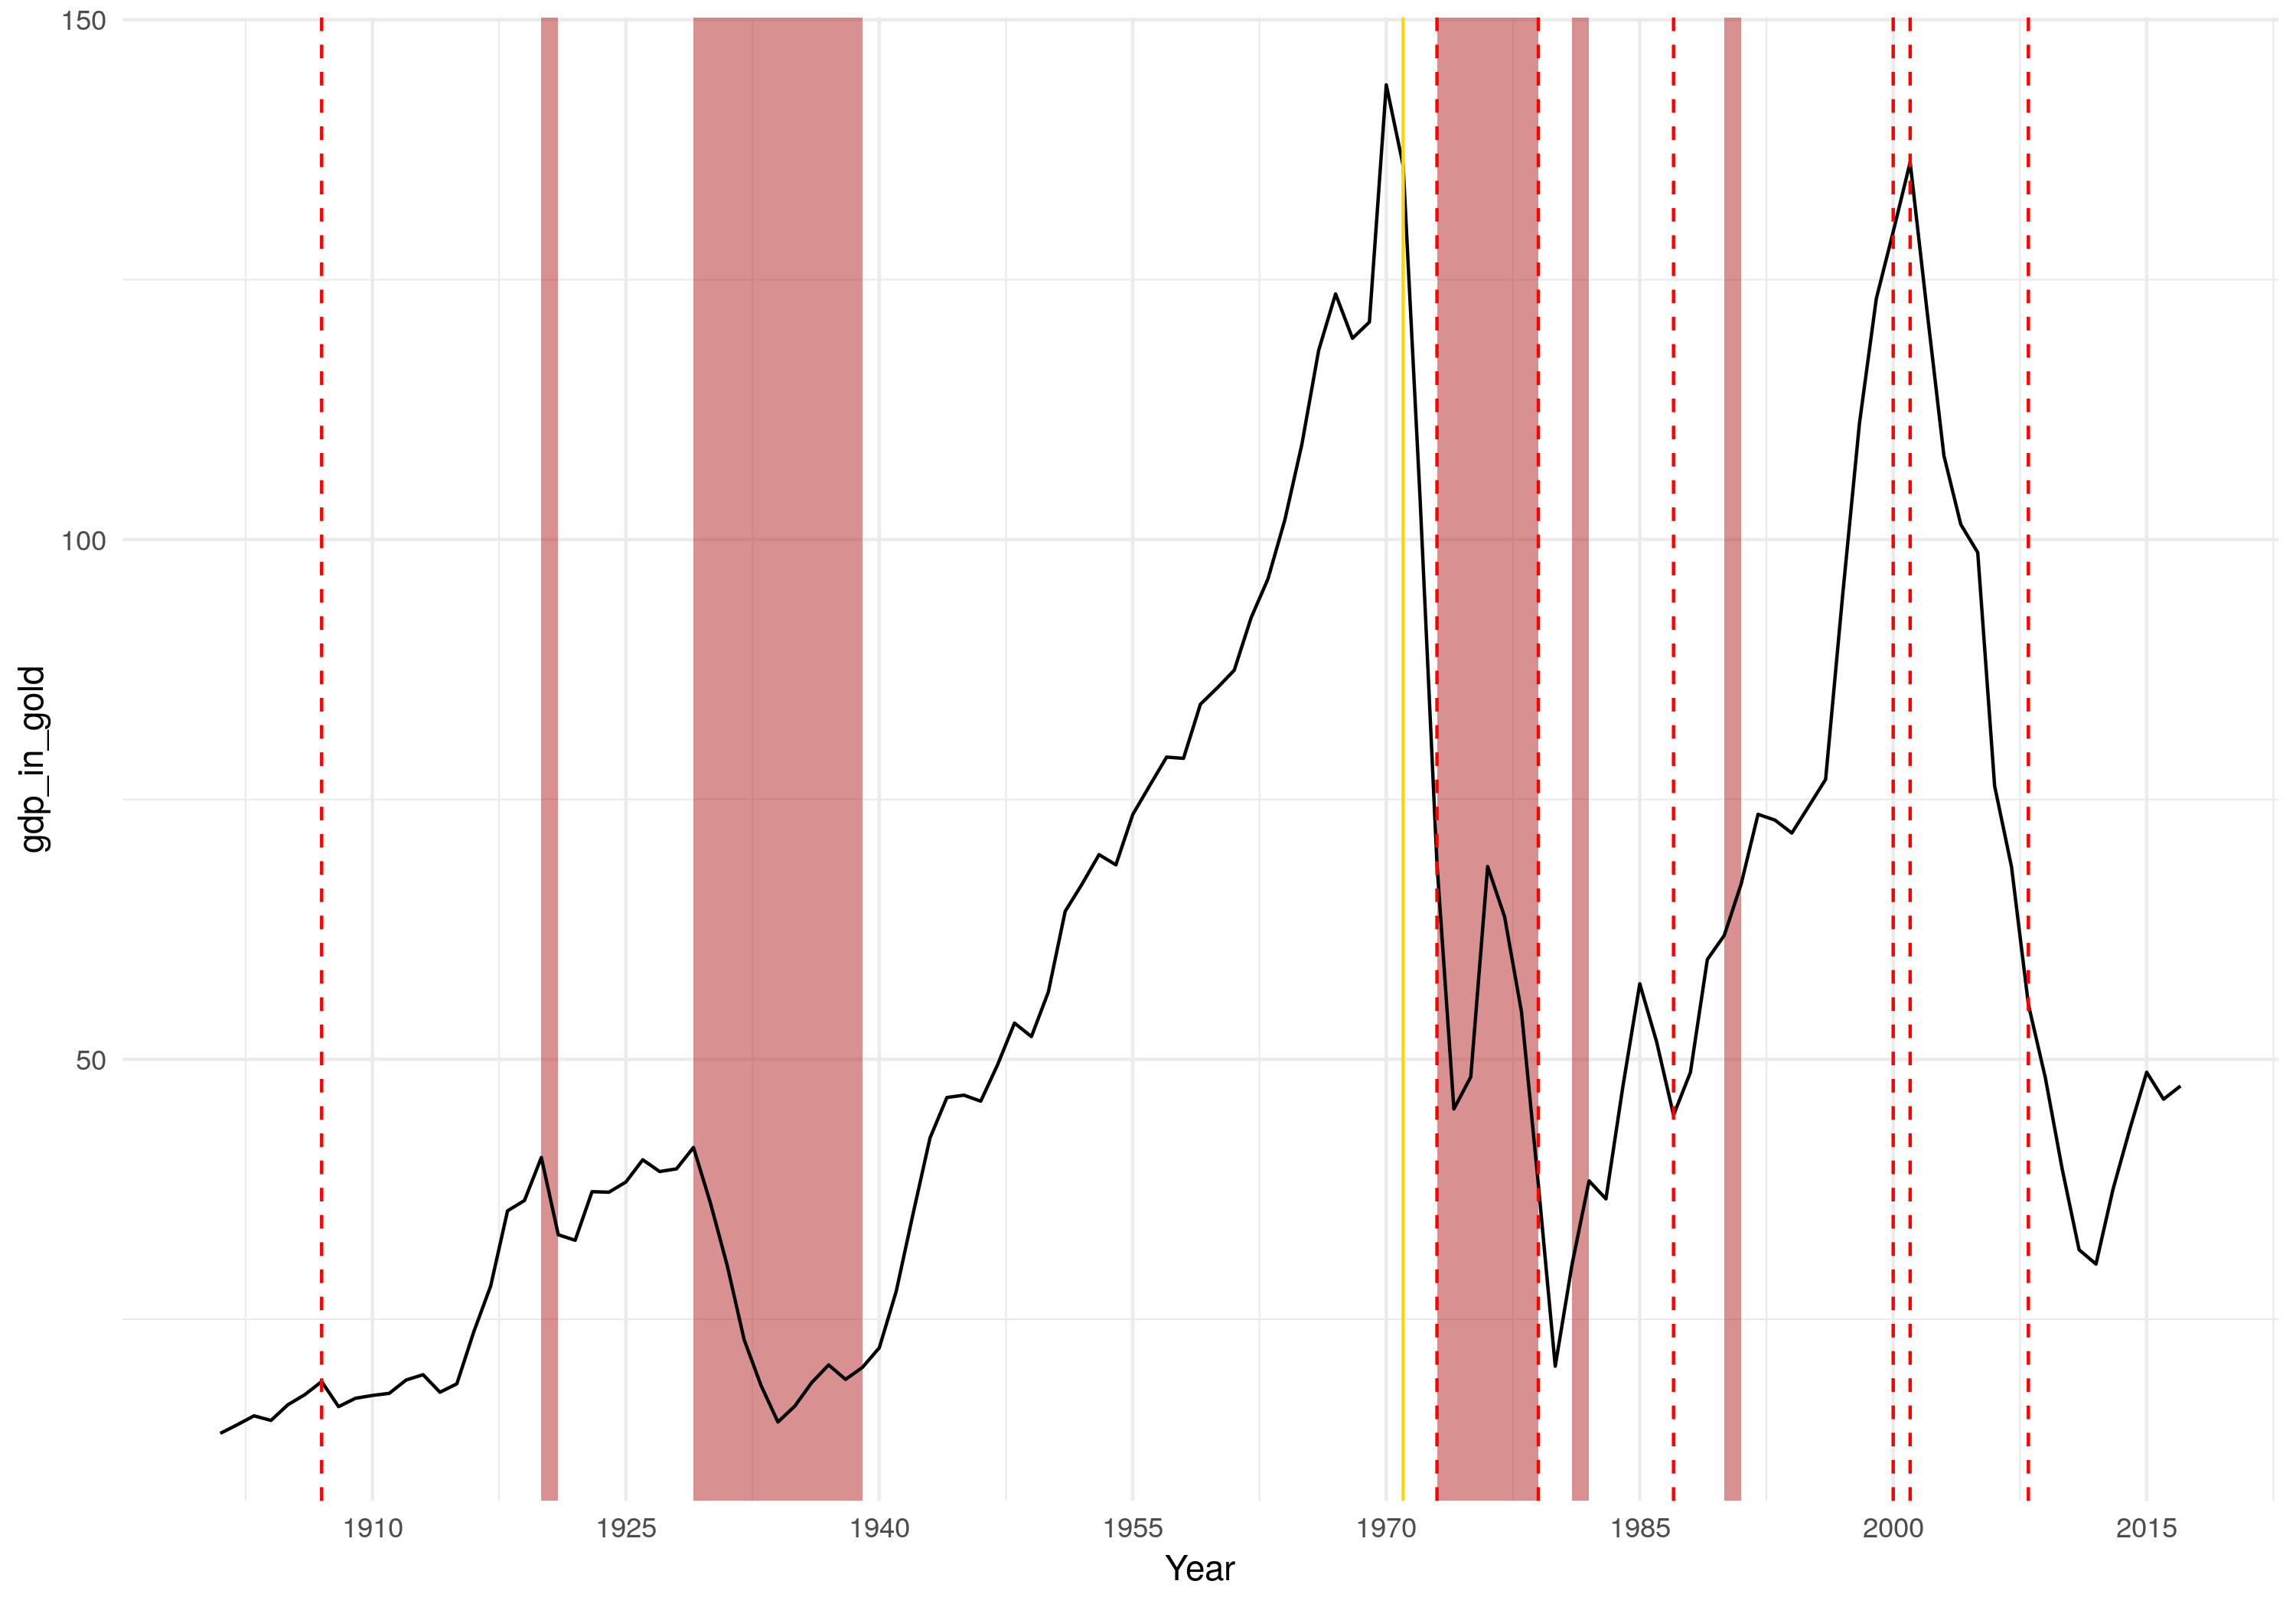
\includegraphics[width=0.75\linewidth]{gdp_in_gold_eda.PNG}
	\label{fig:PBI}}
	\subfigure[]{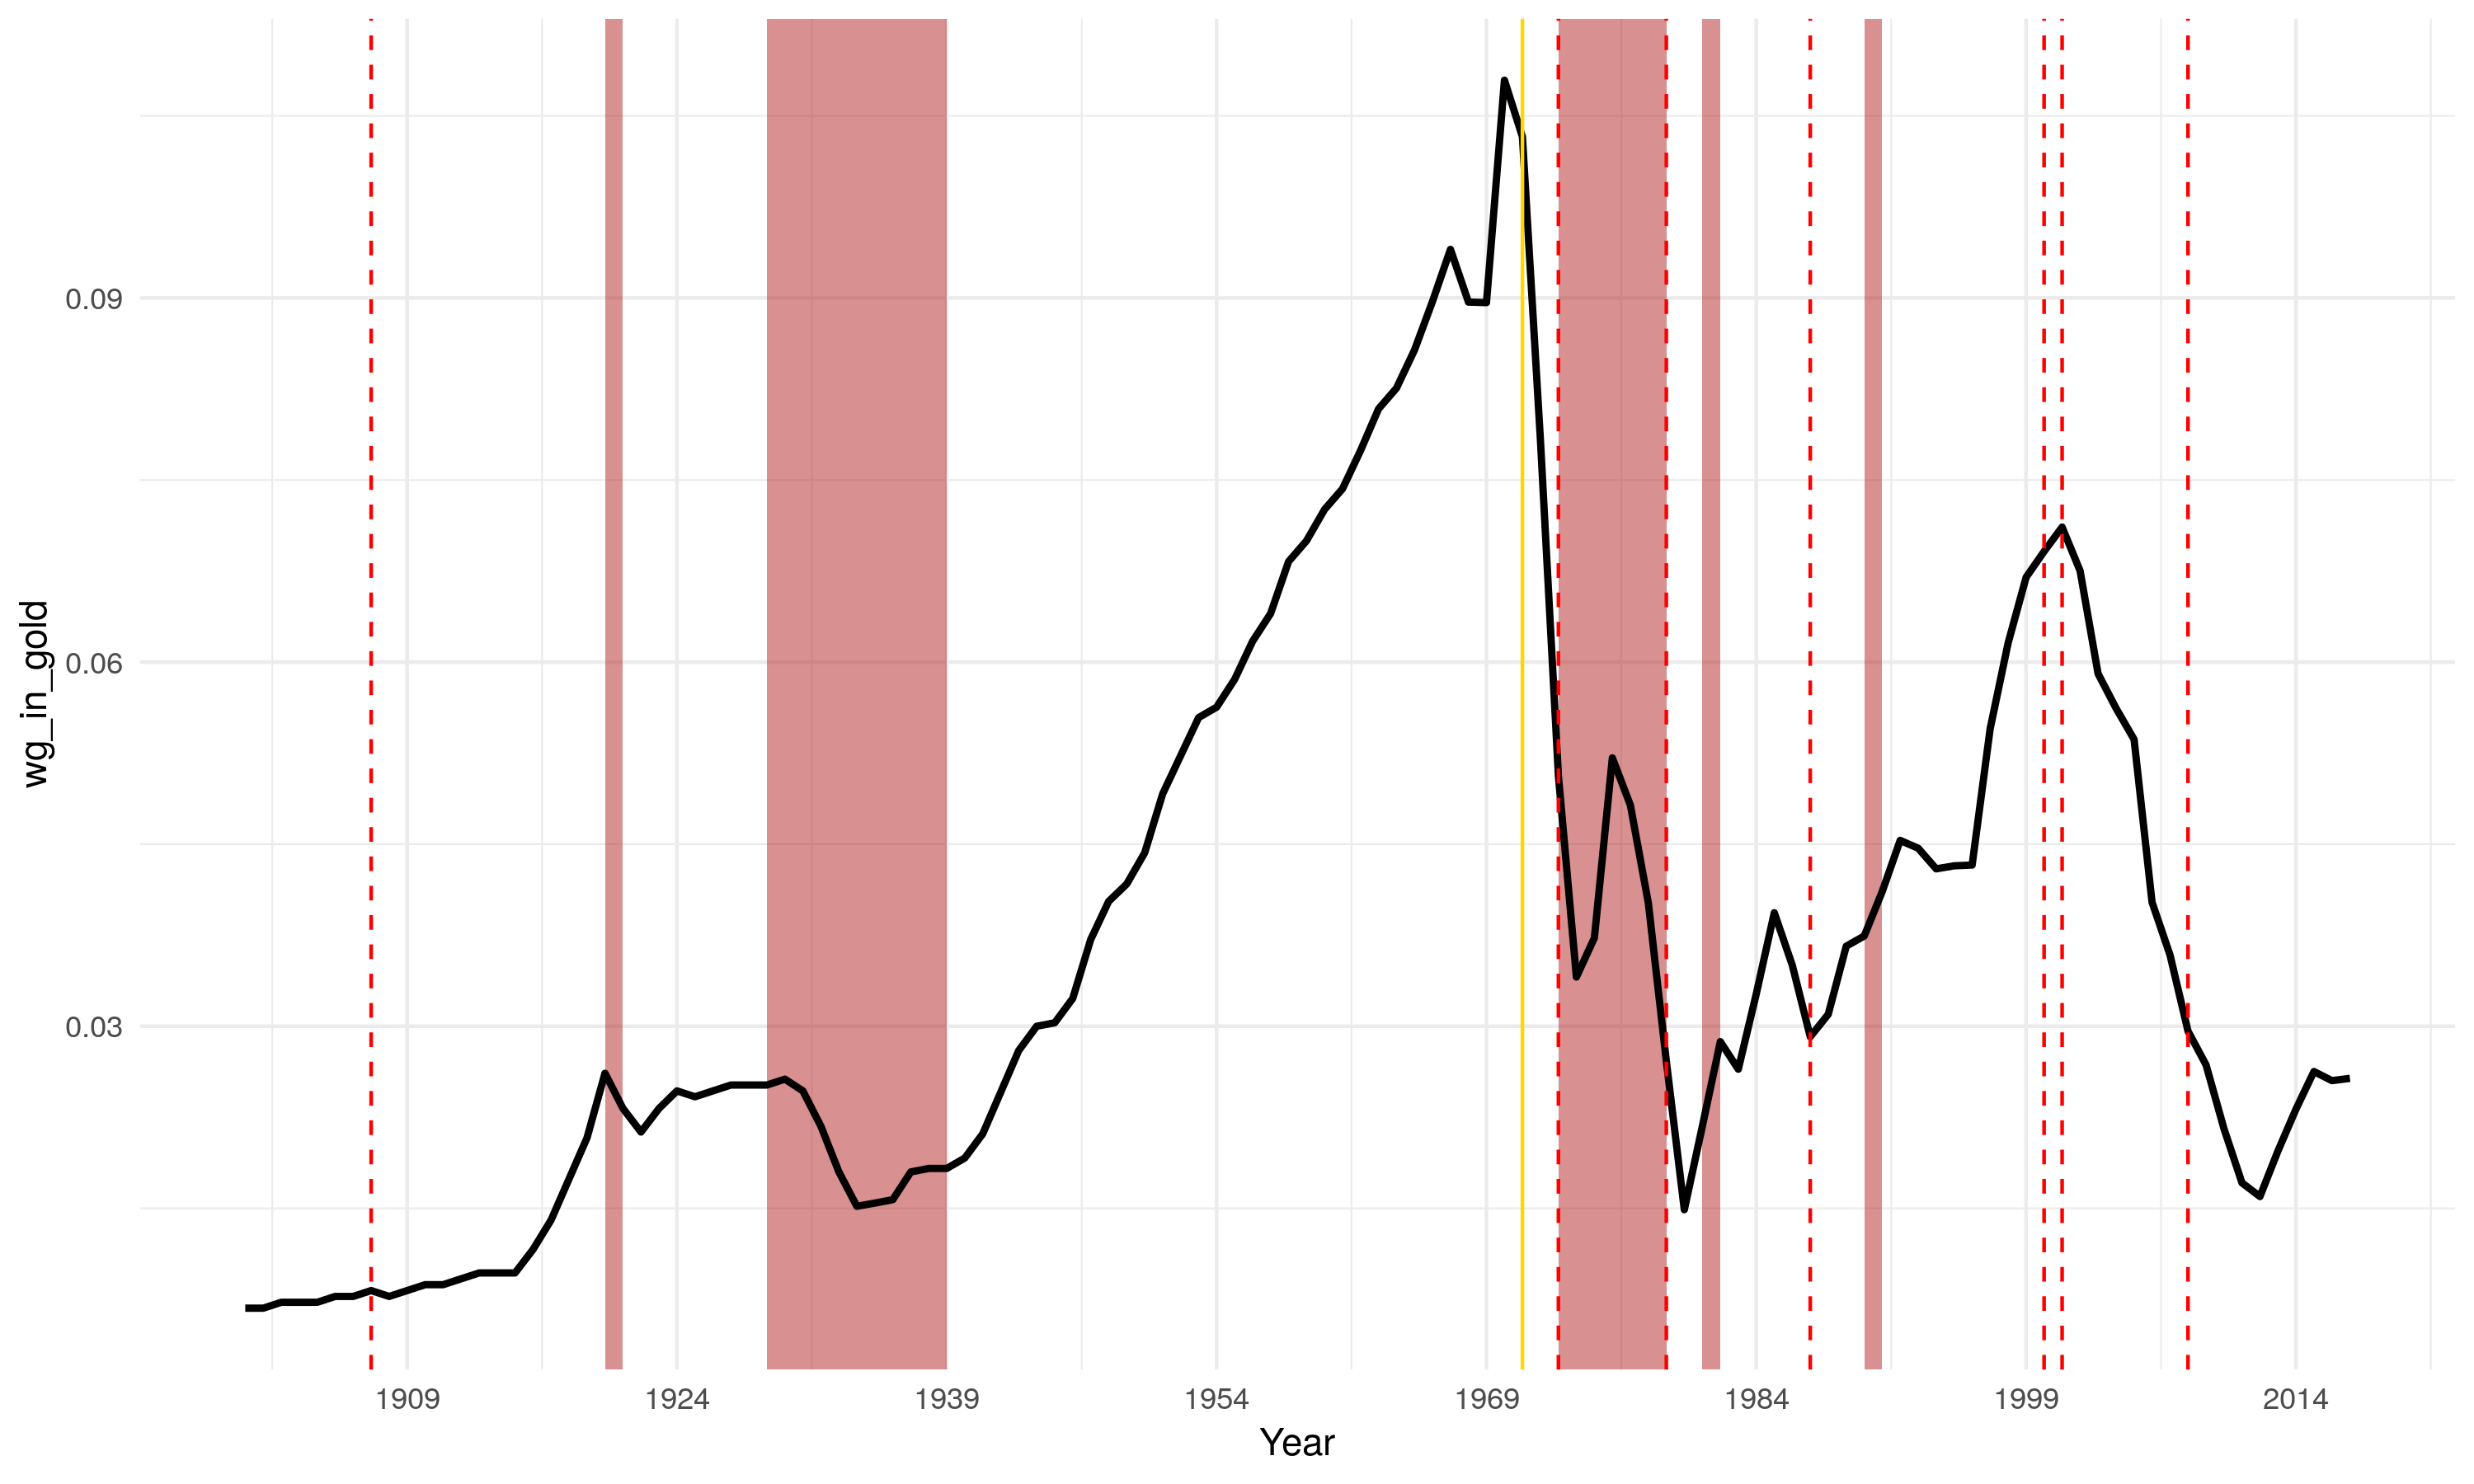
\includegraphics[width=0.75\linewidth]{wg_in_gold_eda.PNG}
	\label{fig:salario}}
	\caption{Series Expresadas en Oro. Destacado de crisis conocidas} \label{fig:series_crisis}
\end{figure}

% latex table generated in R 3.5.1 by xtable 1.8-3 package
% Tue Oct 16 20:07:52 2018
\begin{table}[ht]
	\centering
	\begin{tabular}{ll}
		\hline
		Periodo & Crisis \\ 
		\hline
		1907 & Pánico de 1907 \\ 
		1920 – 1921 & Depresión de 1920 – 21 \\ 
		1929 – 1939 & La gran depresión \\ 
		1970s & 1970s Crisis Energética \\ 
		1973 & Shock de preciso del petróleo de la OPEC(1973) \\ 
		1979 & Revolución Iraní\\ 
		1980s & Recesión de principio de los 80'\\ 
		1987 & Black Monday \\ 
		1990s & Recesión de principio de los 90'\\ 
		2000 & Burbuja de las Dot-com \\ 
		2001 & 911 \\ 
		2008 & Crisis de las subprime \\ 
		\hline
	\end{tabular}
\caption{Principales crisis en EEUU y el mundo.}
\label{tabla_crisis}
\end{table}

In the first place what is observed is the similarity of both series. They Both show three peaks, during the 20', in 1970 and 2000, followed by deep falls. The normalization by the gold-price allows to see a great cycle with three oscillations, at least apparently, during the twentieth century. The crises reviewed by the economic history literature seem to have their correlate in the movements observed in both series. Besides, it is also interesting to note that the third upward movement, whose peak is in the year 2000, leads to a value similar to that of the previous oscillatory movement for the case of GDP, but not for wages. This expresses that the distribution of the GDP between wage and profit has changed in the last period.

To complement the analysis of the United States series, it is interesting to observe the movement of the product at the United Kingdom for the preceding centenaries. During the eighteenth and nineteenth centuries this country was parapet as the core of global accumulation, and therefore it may be possible to find evidence of the economic cycle in this country in particular. The figure \ref{fig:uk_gdp} shows the GDP of the United Kingdom, between 1700 and 1900. It is normalized by the price of gold in the London market from 1718, while the first years correspond to the official British price. At the same time, the years of fall of the GDP from 1800 are stand out, given that for the eighteenth century there are no visually outstanding points.

\begin{figure}[H]
	\centering
	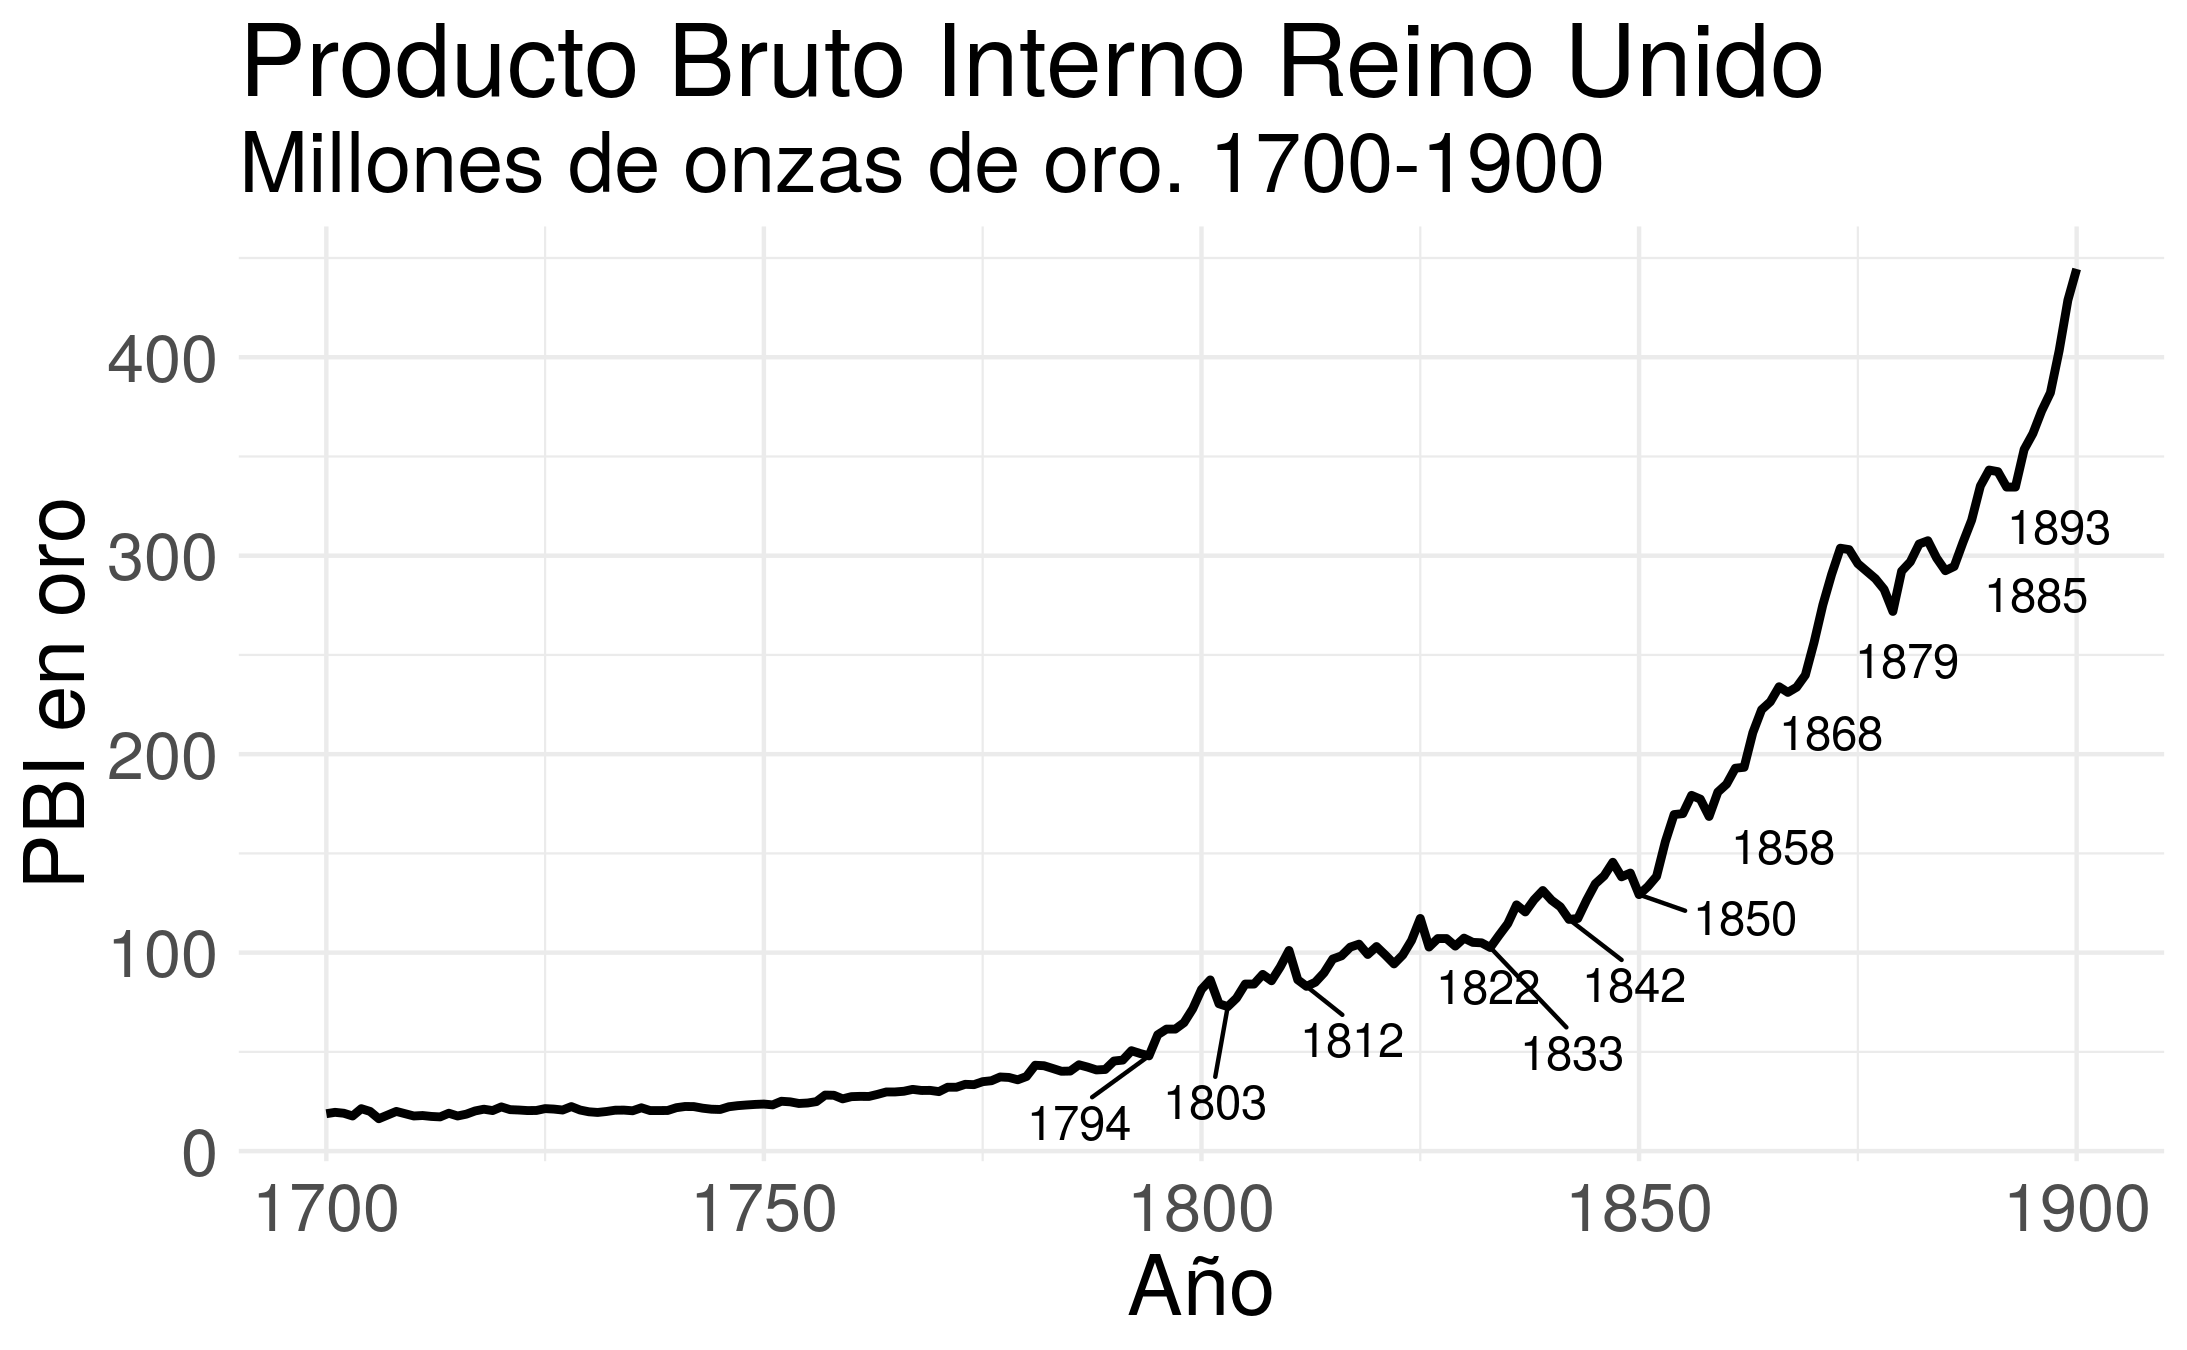
\includegraphics[width=0.75\linewidth]{uk_gdp.png}
	\caption{} 
	\label{fig:uk_gdp}
\end{figure}


What is observed is a softer upward movement than that seen in the 20th century. It is worth mentioning that the movement of the product in the United Kingdom during the twentieth century retains an important similarity with that seen in the case of the United States. In the figure \ref{fig:uk_gdp}, however, a cyclic movement is observed of around 10 years of extension. During the nineteenth century it can be noted that every 7-11 years there is a fall in the product in terms of its ability to buy gold. Just as the twentieth century accounts for three large oscillations, the nineteenth century clearly marks the shorter oscillations, around 10 years, while the eighteenth century in relative terms expresses greater stability.

In the following section, the described series will be used as inputs for a technique coming from the field of signal processing, Wavelets, which allows to highlight automatically the most important cyclic amplitudes of the series.

\section{Wavelets}

Si bien en la econometría es extendido el uso de modelos autoregresivos y de medias móviles para el análisis de series de tiempo, existe en la literatura de análisis de señales otras técnicas de amplia difusión que aún no son de uso generalizado en el estudio de series económicas. Un ejemplo clásico en este sentido son las series de Fourier. En este campo de estudio se analiza como cualquier serie de tiempo se puede pensar como una composición de funciones periódicas, es decir como la suma de senos y cosenos. De esta forma, se construye un espacio de \textit{frecuencia} ($1/periodo$) donde se definen las funciones periódicas en función de su frecuencia (o extensión en el tiempo, movimiento horizontal) y amplitud (movimiento vertical). En la figura \ref{fig:ciclo} se puede observar estas definiciones.

\begin{figure}[H]
	\centering
	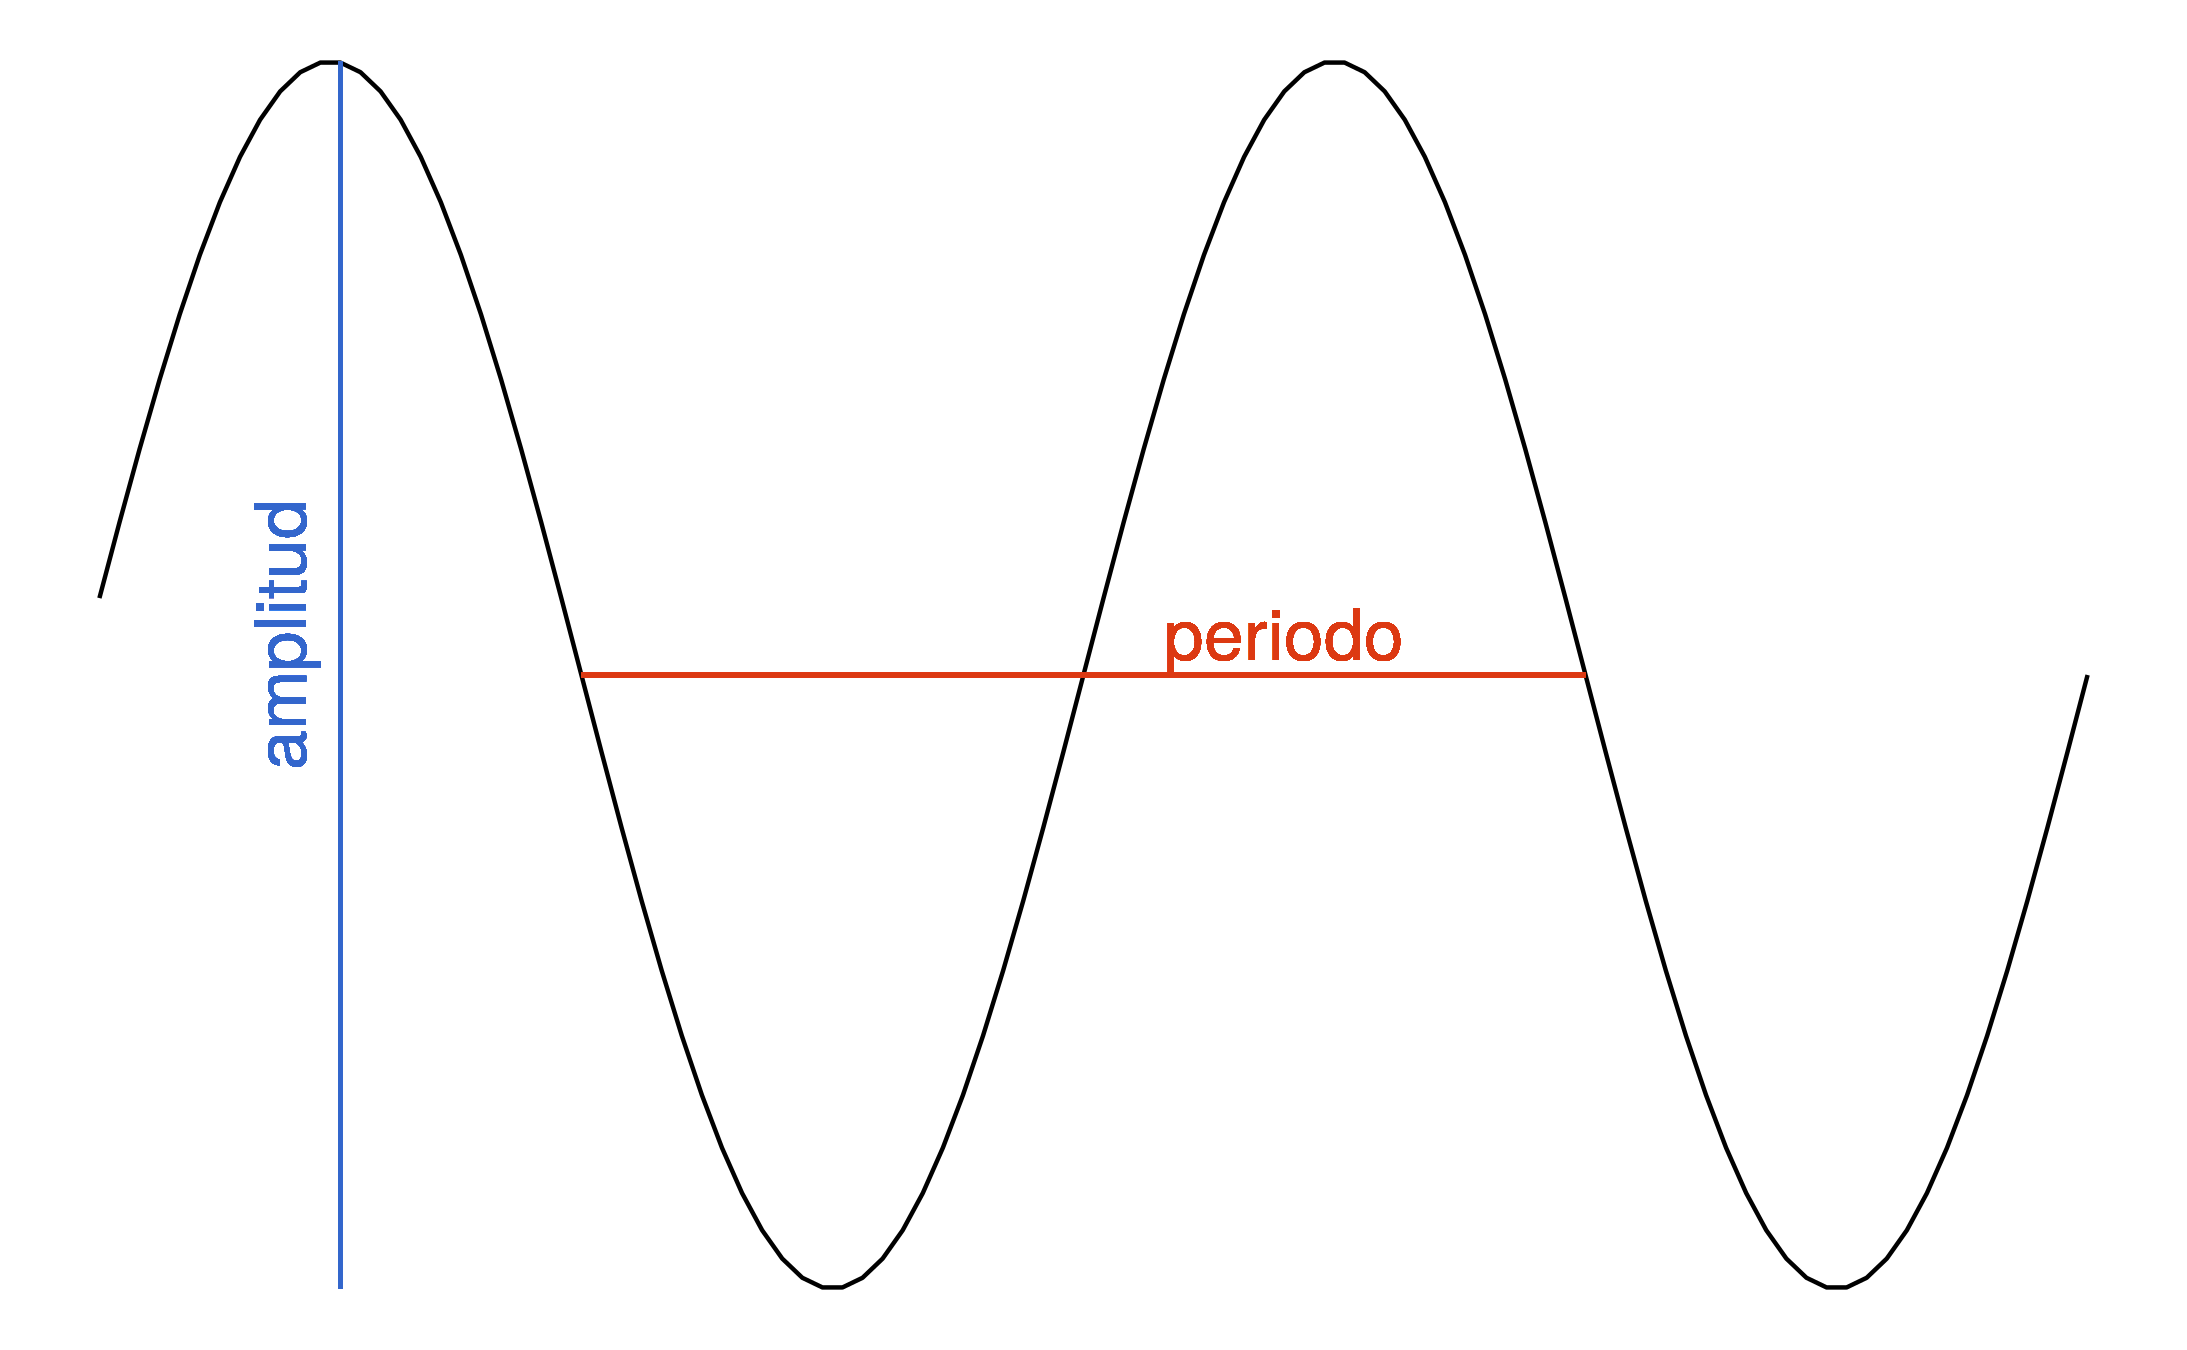
\includegraphics[width=0.65\linewidth]{ciclo.png}
	\caption{período y amplitud} \label{fig:ciclo}
\end{figure}

La descomposición de Fourier se basa en una transformación del dominio de la serie, desde el dominio del tiempo, al dominio de la frecuencia.\\

Las wavelets también son un tipo de transformación sobre la serie original que puede pensarse como una rotación de un espacio de funciones a un dominio diferente. Pero a diferencia de la transformada de fourier que tiene como base de funciones los senos y cosenos, la transformada Wavelet tiene como base de funciones una tipo particular, denominadas Wavelets \cite{castro1995wavelets}. Una base de este tipo se construye a partir de una función madre, que es una onda corta, de duración finita. Es decir, a diferencia de las funciones seno y coseno que se extienden infinitamente, los wavelets tienen \textit{soporte compacto}, es decir que utilizan como base funciones que no se extienden infinitamente en el dominio del tiempo. Otra característica de las funciones wavelet es que el área debajo de la curva debe ser igual a cero, es decir que esta centrada en cero. Esta función madre se traslada y dilata para construir una base ortonormal. 

Mientras que una transformación de Fourier de una serie desde el dominio del tiempo hacia el dominio de la \textit{frecuencia} toma la forma de:

$$
X(F)=\int_{-\infty}^{\infty} x(t) e^{-j2\pi Ft}dt
$$

La transformada wavelet lleva del dominio del tiempo al dominio de \textit{escala} y \textit{traslación}:

$$
X(a,b)=\int_{-\infty}^{\infty} x(t) \psi^*_{a,b}(t)dt
$$

La escala describe la frecuencia (inversa de la extensión o período) del ciclo, mientras que la traslación describe el movimiento a lo largo de la serie. Dado que las series de baja frecuencia (ciclos más largos) ocupan una porción mayor de la serie, son más difíciles de ubicar en un momento particular del tiempo. Por esto último, la resolución en bajas frecuencias es mala en el dominio del tiempo, pero buena en el dominio de la frecuencia, mientras que los ciclos de alta frecuencia tienen alta resolución en el dominio del tiempo, pero menos resolución en el dominio de la frecuencia.Si lo comparamos con las transformadas de fourier, podríamos pensar que ésta tiene muy alta resolución en el dominio de la frecuencia, pero ninguna resolución en el dominio del tiempo. El wavelet logra definir la presencia de una determinada frecuencia en un determinado momento del tiempo.
 

También es posible entender a los Wavelets como un análisis de la correlación entre una serie de tiempo, y una cierta función ondulatoria compacta, en un momento del tiempo y una frecuencia determinada. Las traslaciones lo que generan es un corrimiento de la función ondulatoria, y por lo tanto podemos calcular la correlación para todo el rango temporal. El reescalado modifica la frecuencia de la función ondulatoria, lo que permite calcular la correlación para varias frecuencias de onda diferentes. La cantidad de datos disponibles es la que define la capacidad de reescalar la función base, es decir, cuan bajas son las frecuencias mínimas que se puede analizar. Finalmente lo que obtenemos es un valor de la asociación lineal entre la serie original y la función base, para cada valor del tiempo y la frecuencia.  

La función base que utilizamos para el presente trabajo es la denominada \textit{Morlet Wavelet}, que tal como se implementa en la librería WaveletComp \citep{Roesch2018} tiene la siguiente forma funcional:
$$
\psi(t)=\pi^{-\frac{1}{4}}e^{i\omega t}e^{\frac{-t^2}{2}}
$$

Donde $\omega$ es la frecuencia angular (tasa de rotación en radianes por unidad de tiempo). Esta es una función continua, compleja, frecuentemente utilizada en la literatura \citep{conraria2011continuous}. Por su parte, las base a partir de la traslación, $a$, y el escalado, $b$, implementada es:

$$
X(a,b)=\sum_{t} x(t)   \frac{1}{b} \psi^*\left(\frac{t-a}{b}\right)dt
$$

Visualmente, las traslaciones y reescalados de la función base se pueden observar en la figura \ref{fig:morlet}. Allí se aprecia que las traslaciones se definen en el dominio del tiempo, mientras que los reescalados lo hacen en el dominio de la frecuencia. Luego, si se reconstruye el plano tiempo-frecuencia y se calcula la correlación de cada punto del dicho plano con la serie original, se obtiene una nueva dimensión que representa el grado de ajuste de nuestra serie a cada frecuencia, para los distintos momentos del tiempo. 

\begin{figure}[H]
	\centering
	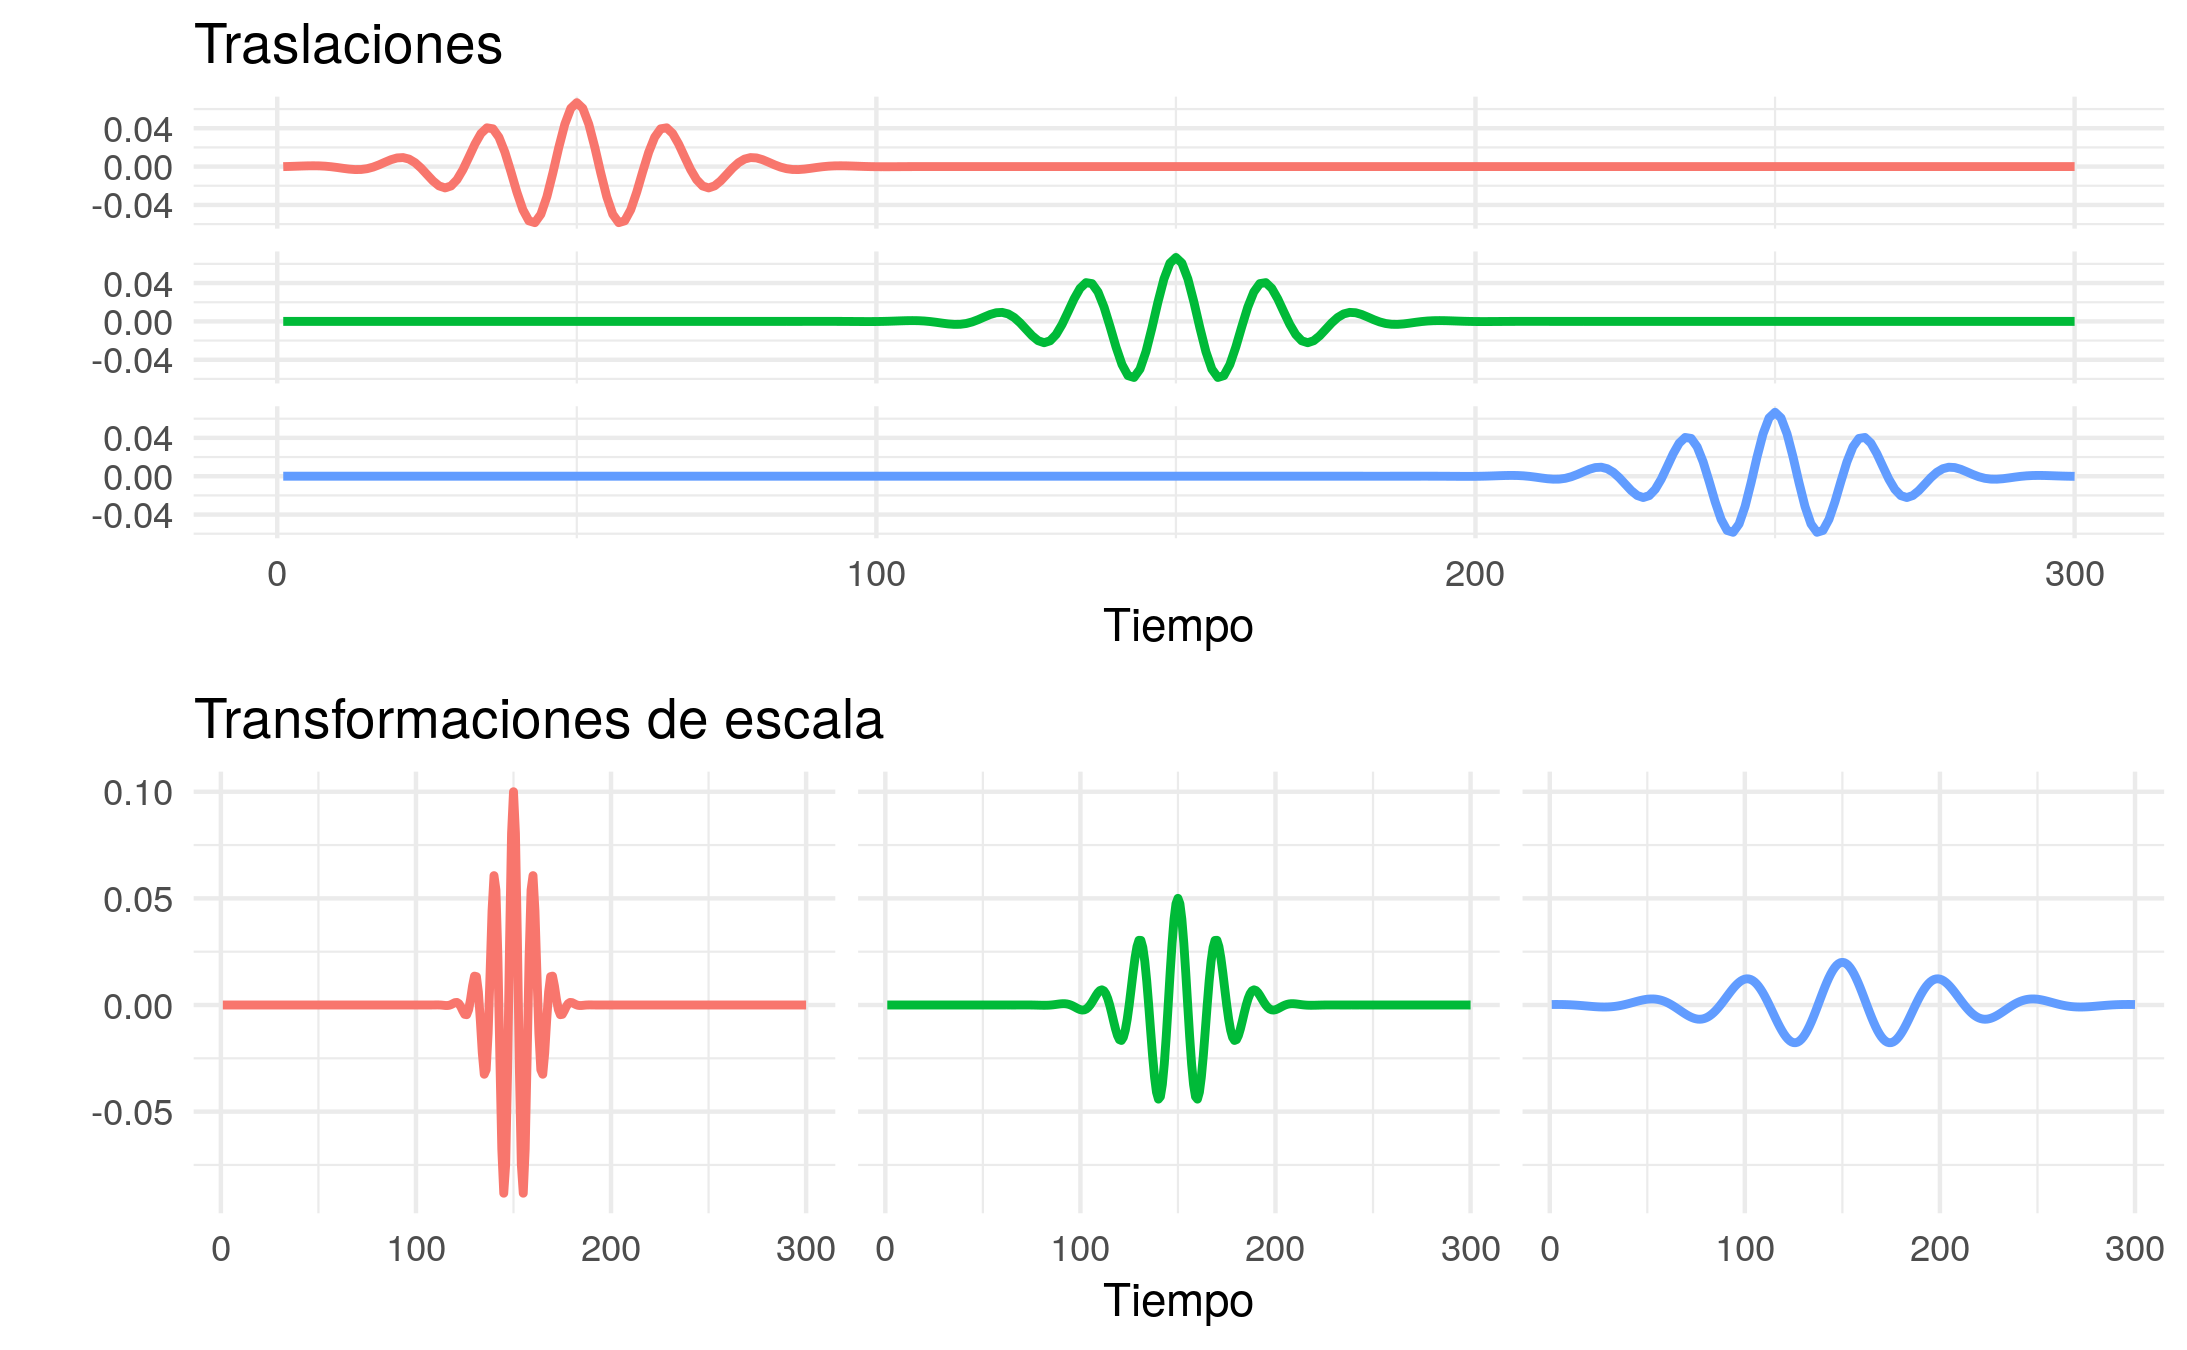
\includegraphics[width=\linewidth]{morelt.png}
	\caption{Traslaciones y reescalados de la función base Morlet} \label{fig:morlet}
\end{figure}


Finalmente, los resultados los podemos visualizar en un \textit{espectograma}, es decir, podemos ver para cada frecuencia, en cada momento del tiempo, el grado de correlación de la serie original con la función morlett en dicho punto.


Para visualizar las wavelets en el análisis del ciclo económico es útil definir un modelo teórico de una economía cíclica, con los diferentes componentes vistos por separado y en su composición, para observar las características del espectograma en este modelo,  y luego compararlo con los datos reales. 
En la figura \ref{fig:serie_teorica} se observan 100 valores de los distintos componentes con los que construiremos la serie, los mismos son:

\begin{itemize}
	\item \textbf{impulso}: Una serie con un valor constante de 50, que en período en particular tomar el valor 100.
	\item \textbf{Tendencia}: Crece medio punto por período.
	\item \textbf{ciclo corto}: Un ciclo de amplitud y extensión pequeña
	\item \textbf{ciclo medio}: Un ciclo de amplitud y extensión media
	\item \textbf{ciclo largo}: Un ciclo de amplitud y extensión grande
	\item \textbf{ruido}: Ruido generado a partir de una distribución normal, poco significativo respecto a la amplitud de los ciclos y la pendiente de la tendencia.
\end{itemize}

En código R, los elementos de la serie teórica se pueden expresar de la siguiente manera:

\begin{lstlisting}
n = 1000
impulso= c(rep(50,(n/2-1)),100,rep(50,n/2))
tendencia = c(1:n)/2
corto = 10 * sin(( 2 * pi/3 ) * c(1:n))
medio = 20 * sin(( 2 * pi/10) * c(1:n))
largo = 30 * sin(( 2 * pi/50) * c(1:n))
ruido <- rnorm(n)
serie_compuesta = impulso + tendencia + corto + medio + largo + ruido
\end{lstlisting}


\begin{figure}[H]
	\centering
	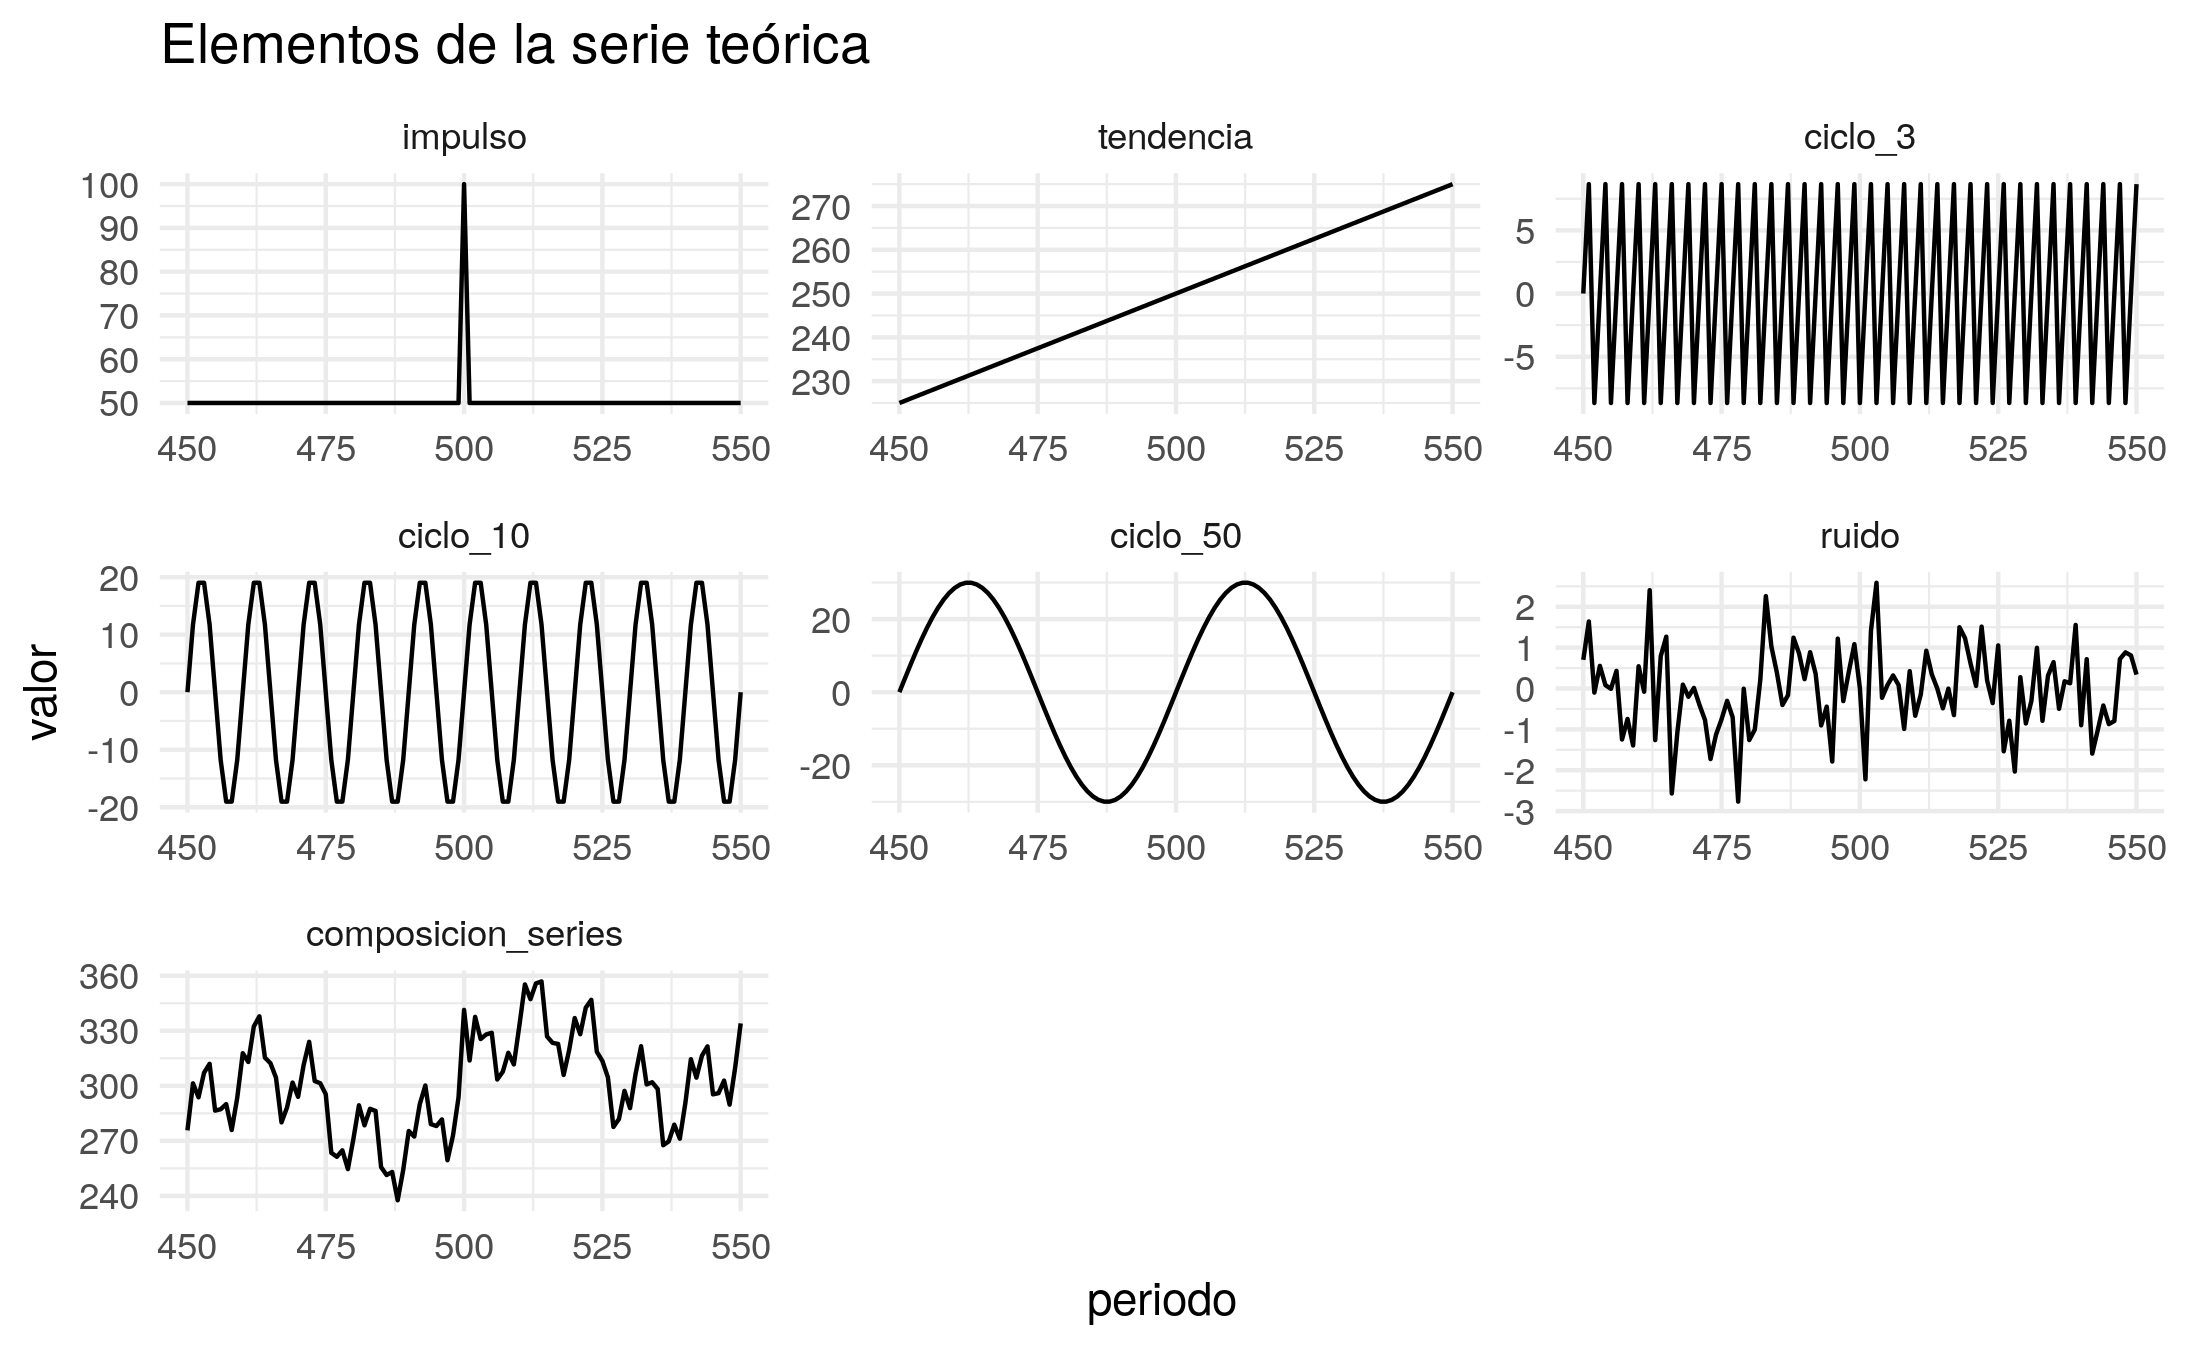
\includegraphics[width=\linewidth]{serie_teorica.PNG}
	\caption{} \label{fig:serie_teorica}
\end{figure}

En la figura \ref{fig:espect_teo} se observa el espectograma de cada uno de los elementos mencionados. Dicho gráfico muestra en el eje vertical el período, la inversa de la frecuencia de onda, que corresponde a la distancia entre los valles o picos de un ciclo. La escala cromática (de los azules para los valores más bajos a los rojos en los valores más altos) representa la amplitud del ciclo. el eje horizontal representa el tiempo calendario. Es decir, para cada tiempo calendario podemos observar la amplitud del ciclo en cada una de las posibles frecuencias de onda. 

\begin{figure}[H]
	\centering
	\subfigure[impulso]{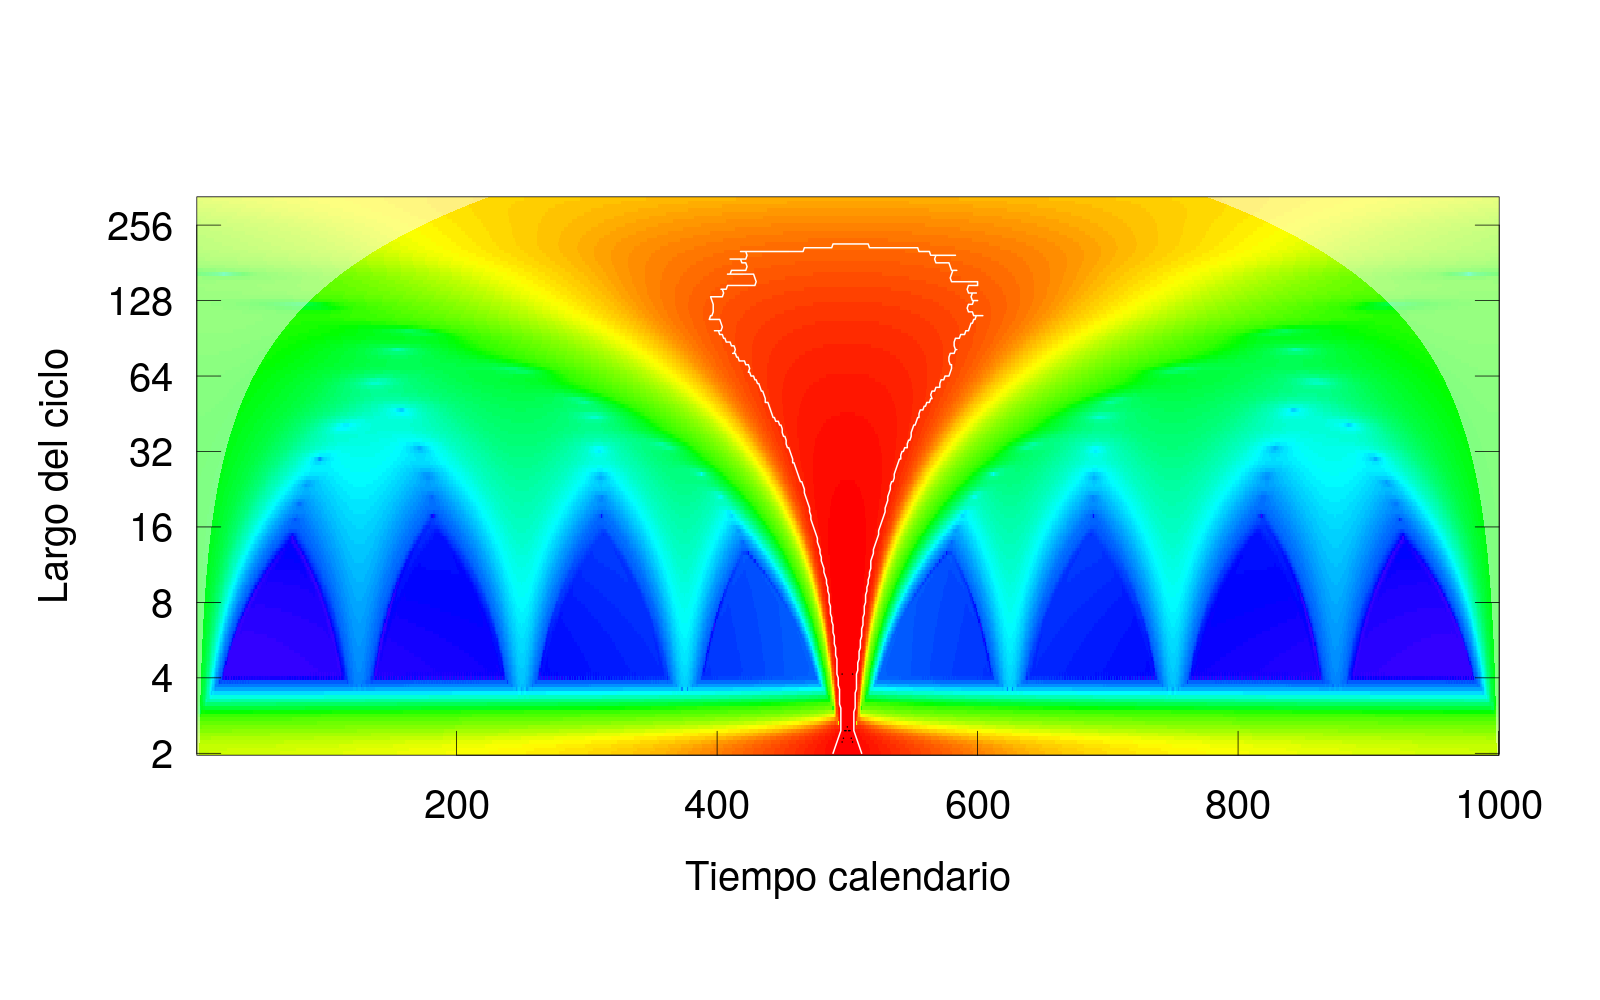
\includegraphics[width=0.49\linewidth]{espectograma_teorico_impulso.png}}
	    \vspace{0.00mm}
	\subfigure[tendencia]{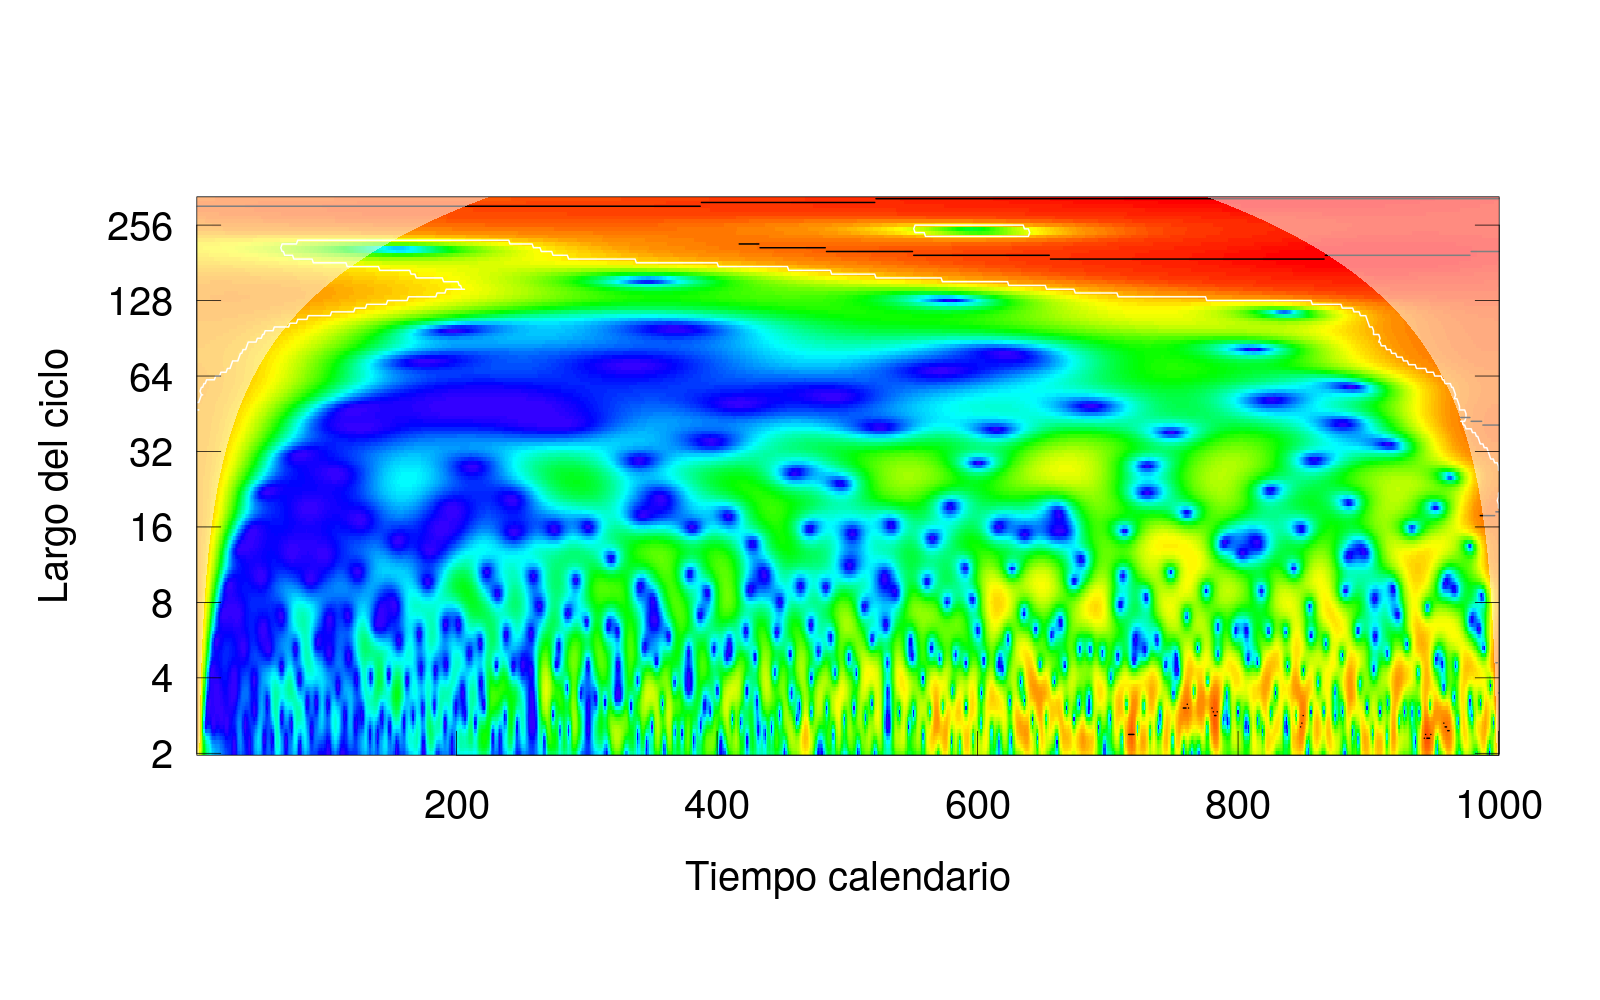
\includegraphics[width=0.49\linewidth]{espectograma_teorico_tendencia.png}}
	    \vspace{0.00mm}
	\subfigure[ciclo de 3 años]{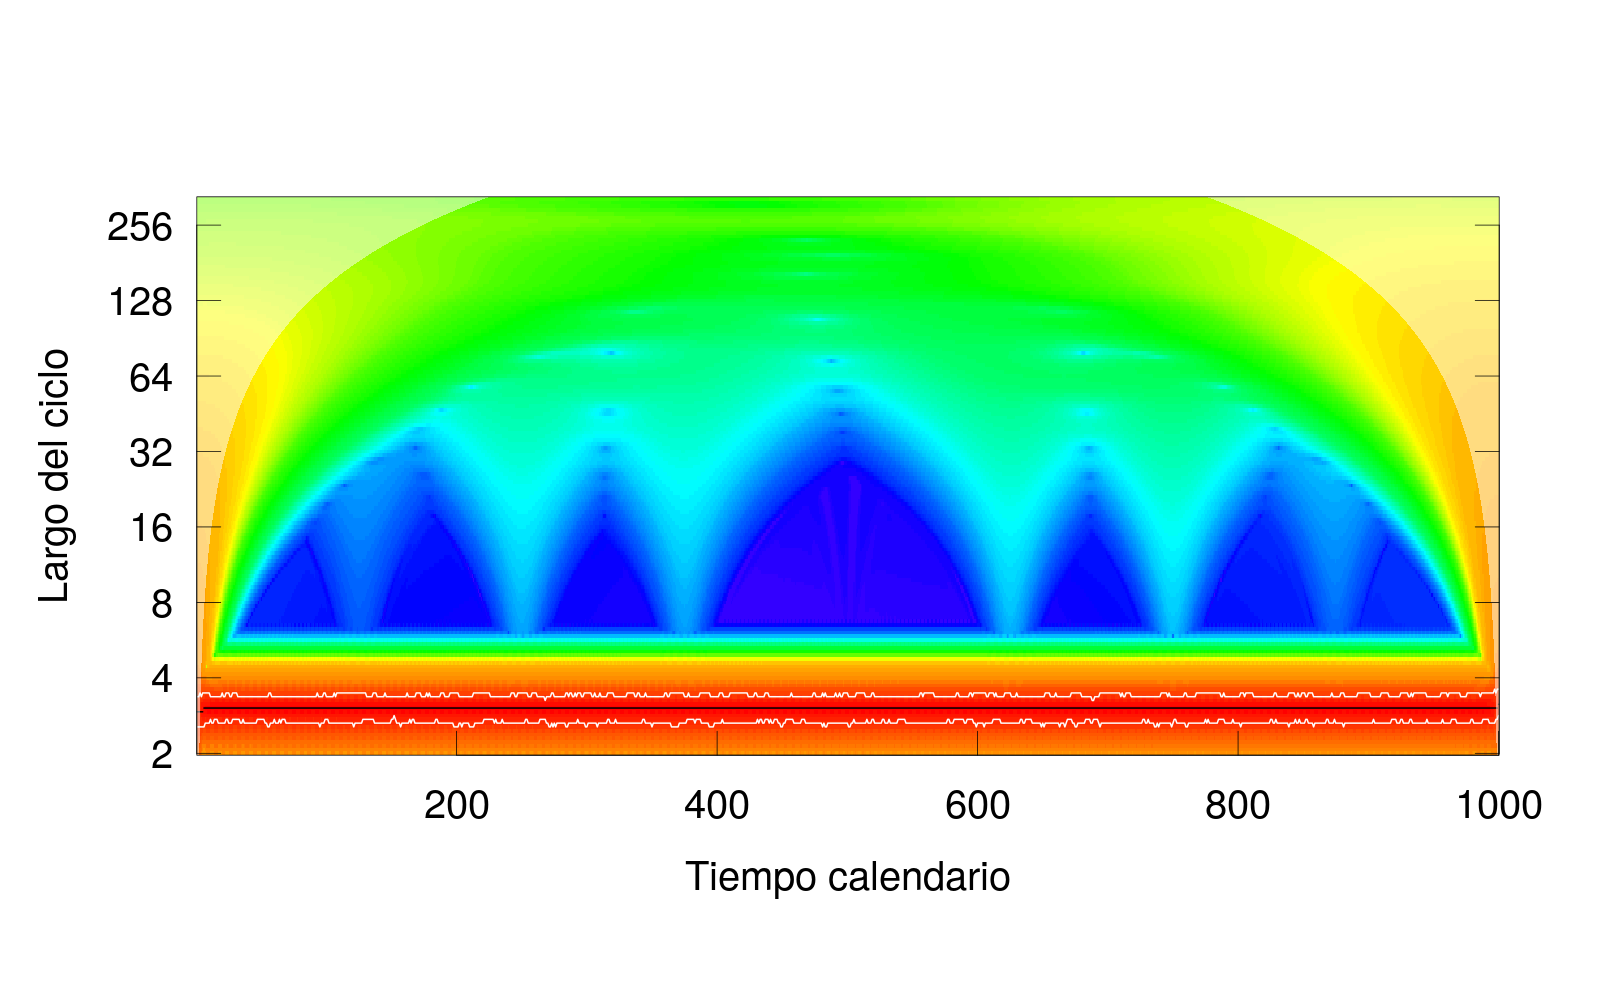
\includegraphics[width=0.49\linewidth]{espectograma_teorico_ciclo_3.png}}
	    \vspace{0.00mm}
	\subfigure[ciclo de 10 años]{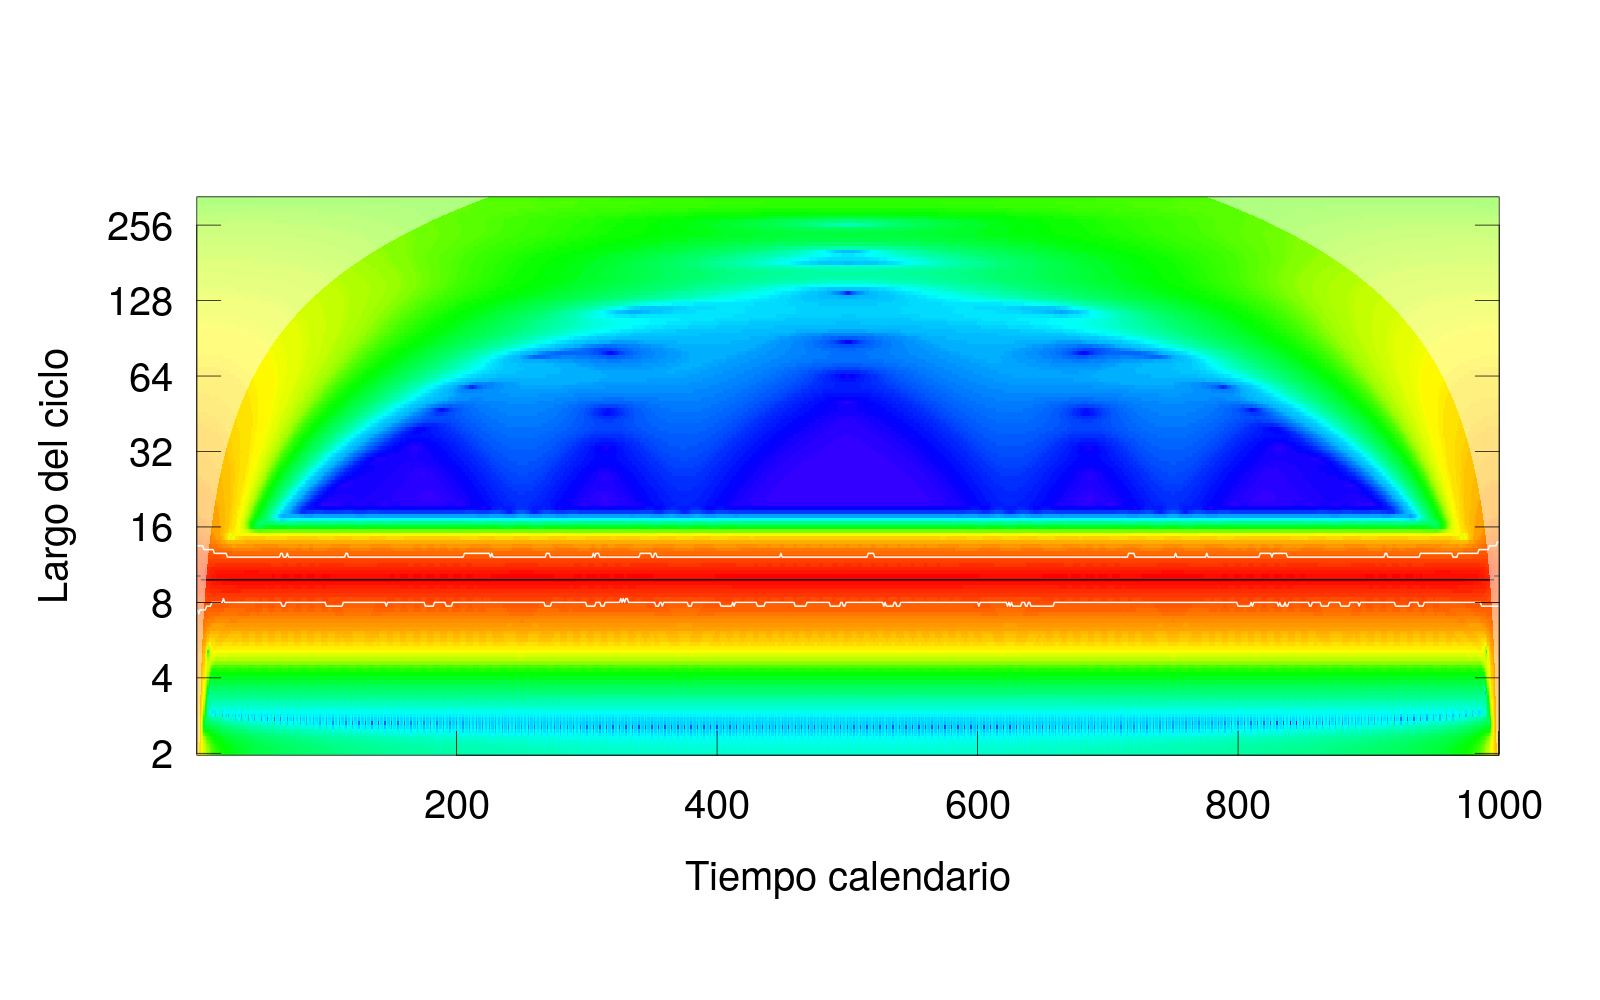
\includegraphics[width=0.49\linewidth]{espectograma_teorico_ciclo_10.png}}
	    \vspace{0.00mm}
	\subfigure[ciclo de 50 años]{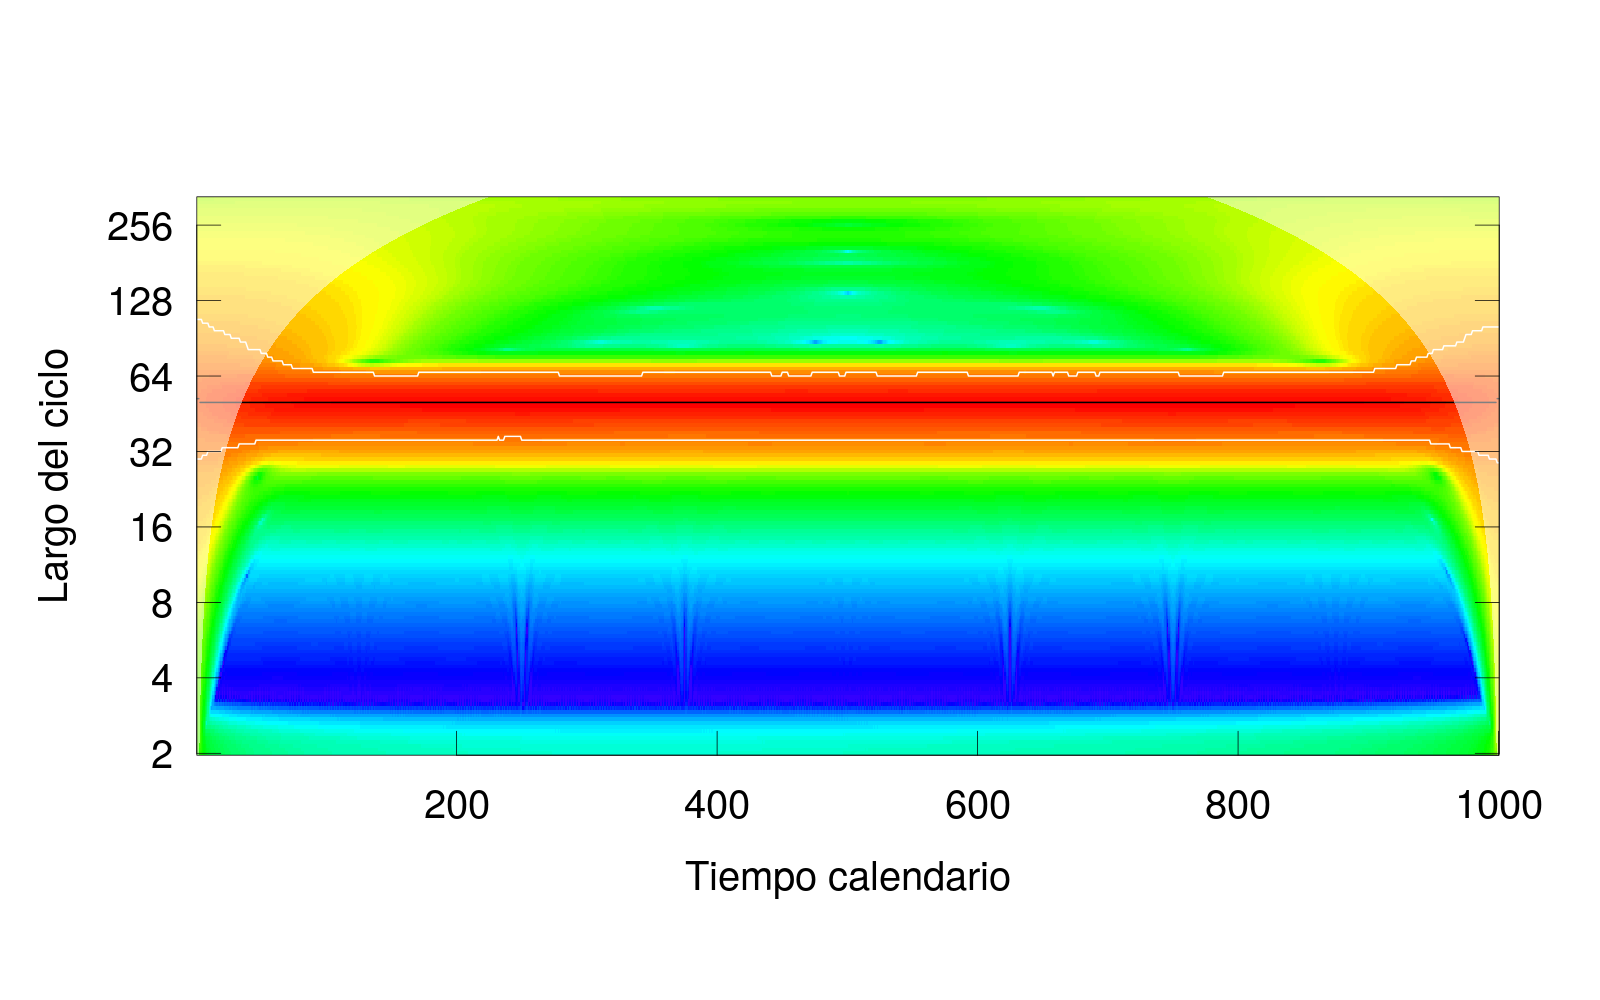
\includegraphics[width=0.49\linewidth]{espectograma_teorico_ciclo_50.png}}
	    \vspace{0.00mm}
	\subfigure[ruido normal]{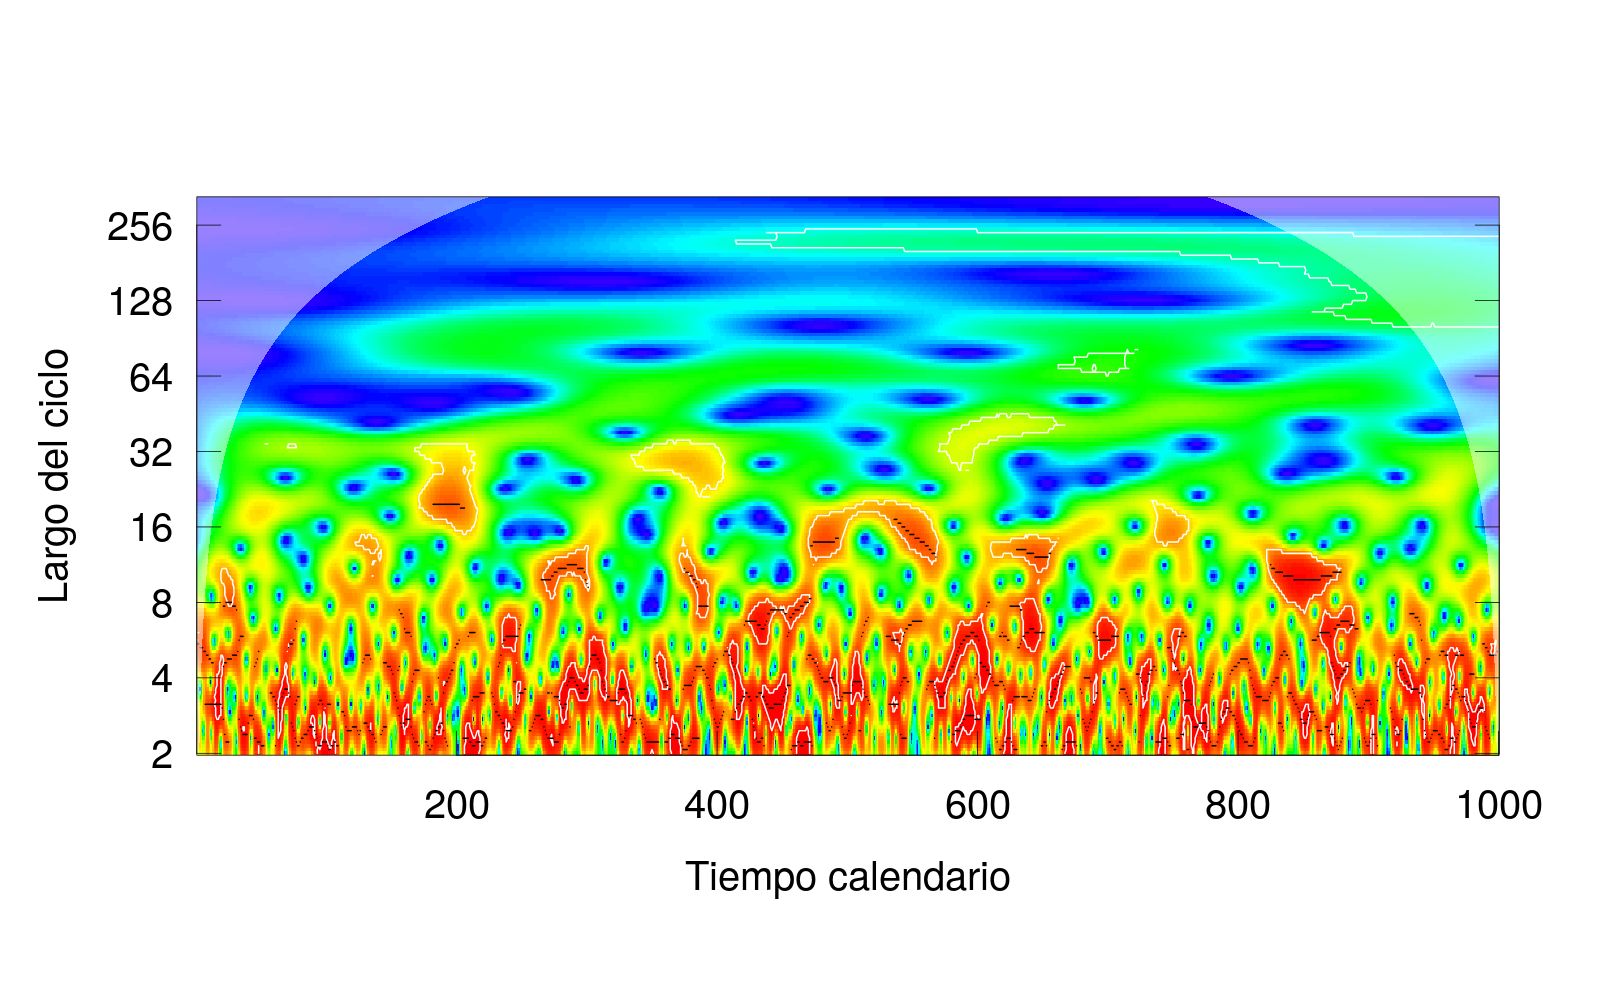
\includegraphics[width=0.49\linewidth]{espectograma_teorico_ruido.png}}
	    \vspace{0.00mm}
	\subfigure[composición de series]{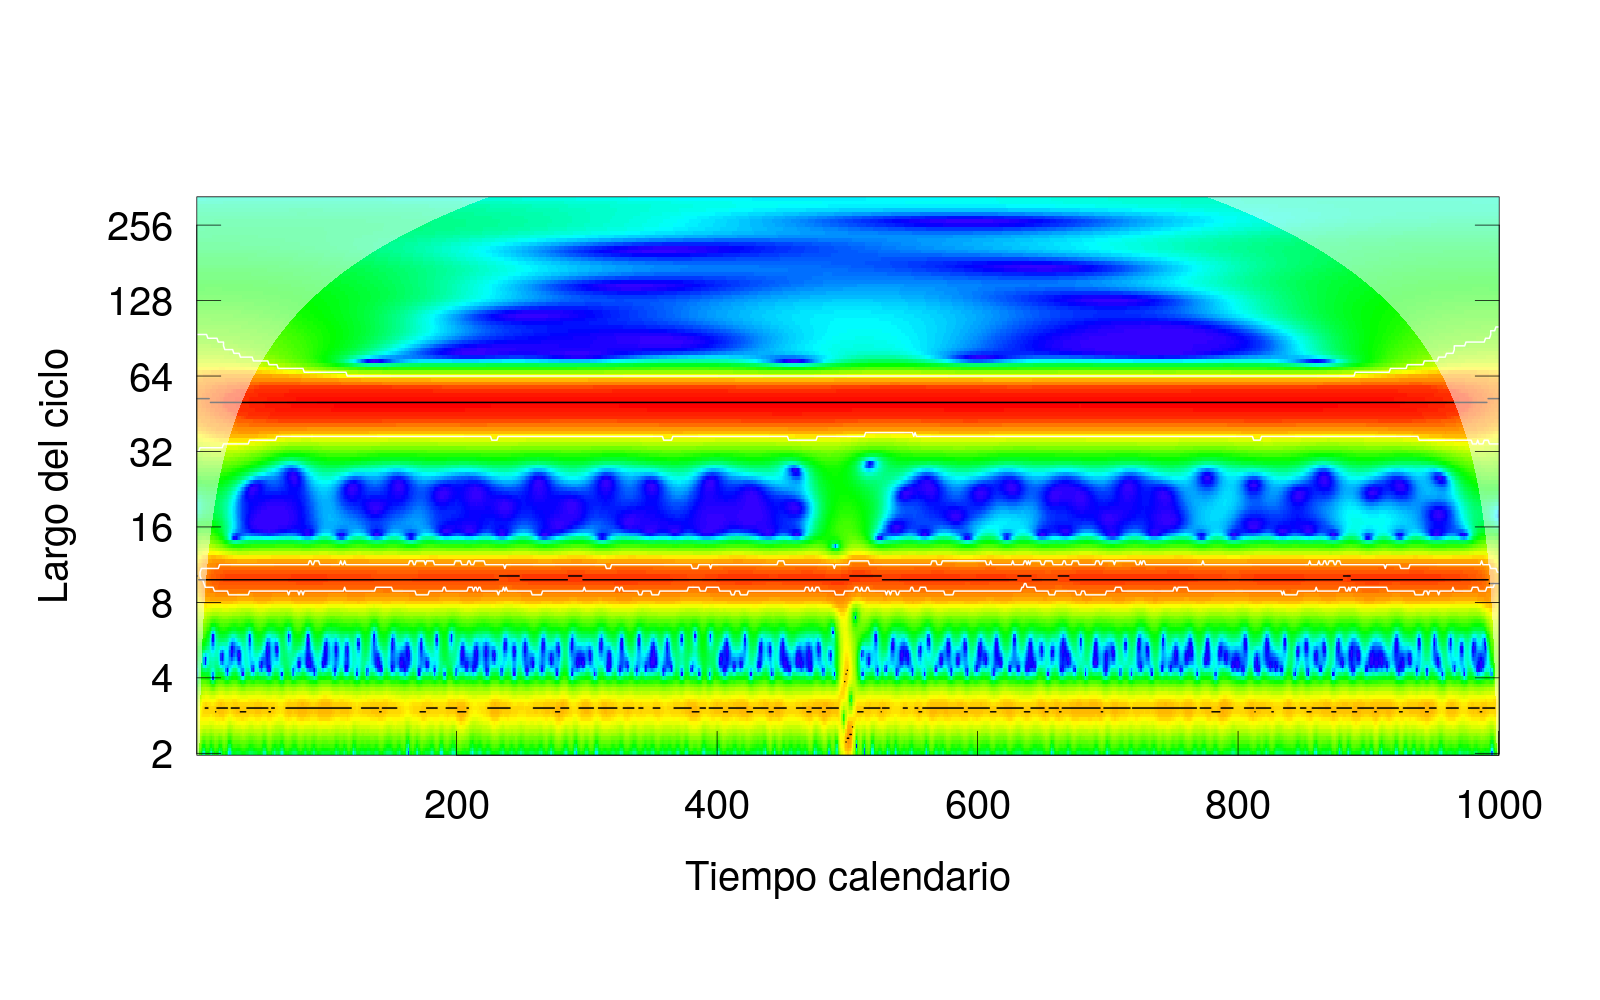
\includegraphics[width=0.75\linewidth]{espectograma_teorico_composicion_series.png}}
	\caption{Espectogramas teóricos} \label{fig:espect_teo}
\end{figure}

Como se observa en la figura \ref{fig:espect_teo} el impulso se presenta como un ciclo de amplitud grande en todas las frecuencias, en el momento correspondiente al salto. La tendencia, por su parte, se presenta básicamente como ruido, dado que es estrictamente un comportamiento no cíclico. Sin embargo, presenta la particularidad de tomar valores de amplitud mayores hacia el final del período para frecuencias bajas, y valores de amplitud particularmente bajos en las frecuencias altas de los primeros momentos.

Los tres ciclos definidos marcan claramente una línea horizontal en el correspondiente período, que luego se diluye hacia las demás frecuencias. Finalmente, el ruido normal presenta un comportamiento muy particular, mostrando mayores amplitudes, de forma irregular, en las frecuencias altas, y homogeneizándose hacia un valor de amplitud baja en los ciclos más largos. Esto se debe a que el ruido normal se puede parecer a un ciclo de períodos muy cortos debido a una sucesión de subas y bajas, pero dado que es un proceso aleatorio, es cada vez más improbable que se asemeje a ciclos de períodos mayores, siendo que ello implicaría una mayor cantidad de sucesiones de subas y bajas consecutivas. A su vez, tanto en el espectograma del ruido normal como en el de la tendencia se puede apreciar como el gráfico pierde resolución para periodos más largos, como se mencionó anteriormente. 

Por último, en la composición de series se observa como los ciclos de mayor amplitud y frecuencia se expresan en la escala cromática de forma más nítida que los ciclos de menor amplitud y frecuencia. Es importante resaltar que la concordancia entre amplitud y frecuencia es producto de la forma en que construimos las series, dado que esperamos que los ciclos económicos más largos se correspondan también con movimientos de mayor amplitud.

Vale mencionar que la elección para el modelo teórico de estos tres niveles y amplitudes cíclicas no es arbitraria, sino que se corresponde a grandes rasgos con lo considerado por la literatura: \cite{kondratieff1979long} estudia las series largas, de unos 50 años, mientras que \cite{kuznets1930secular} propone movimientos seculares de entre 15 y 25 años. Finalmente el Real business cycle \citep{kydland1982time} considera un ciclo corto.



Con lo analizado de la figura \ref{fig:espect_teo} podemos observar los resultados de las series originales. En la figura \ref{fig:espect_PBI_a} se puede observar el espectograma correspondiente al PBI de Estados Unidos expresado en oro. Allí se marca claramente la diferencia en la serie antes y después del 1900, y en particular también se marca el quiebre estudiado de los años 70'. No obstante lo cual, para ese período se observan 3 frecuencias donde se registra un comportamiento cíclico, en los períodos aproximados de 8 y 50 años, y un ciclo diferenciado de este último, de aproximadamente 30 años. Dada la heterocedasticidad de las series, en \ref{fig:espect_PBI_b} se propone el espectograma de la misma serie tomada en logaritmo de base 10. De esta forma lo que se observa es que el ciclo de 50 años se extiende más allá en el tiempo, hasta mediados del Siglo XIX. Por su parte, aparece brevemente un ciclo más corto, de aproximadamente tres años, en la década del 70.

\begin{figure}[H]
	\centering
	\subfigure[PBI]{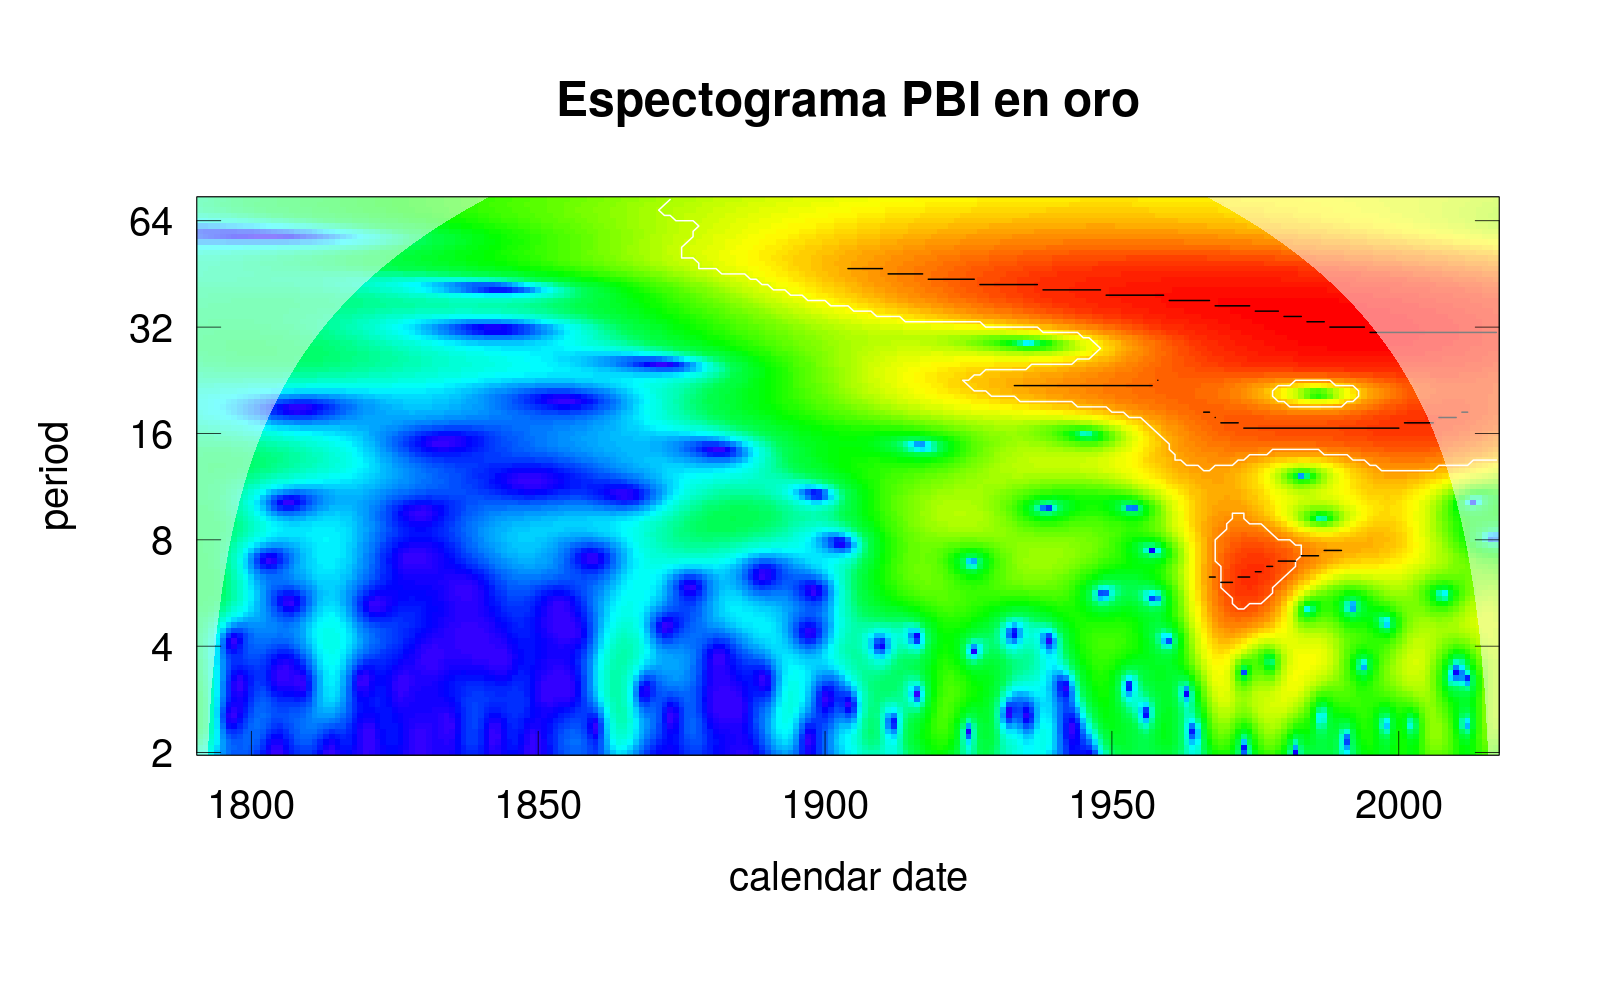
\includegraphics[width=0.75\linewidth]{espectograma_gdp.png}
	\label{fig:espect_PBI_a}}
	\subfigure[$log(PBI)$]{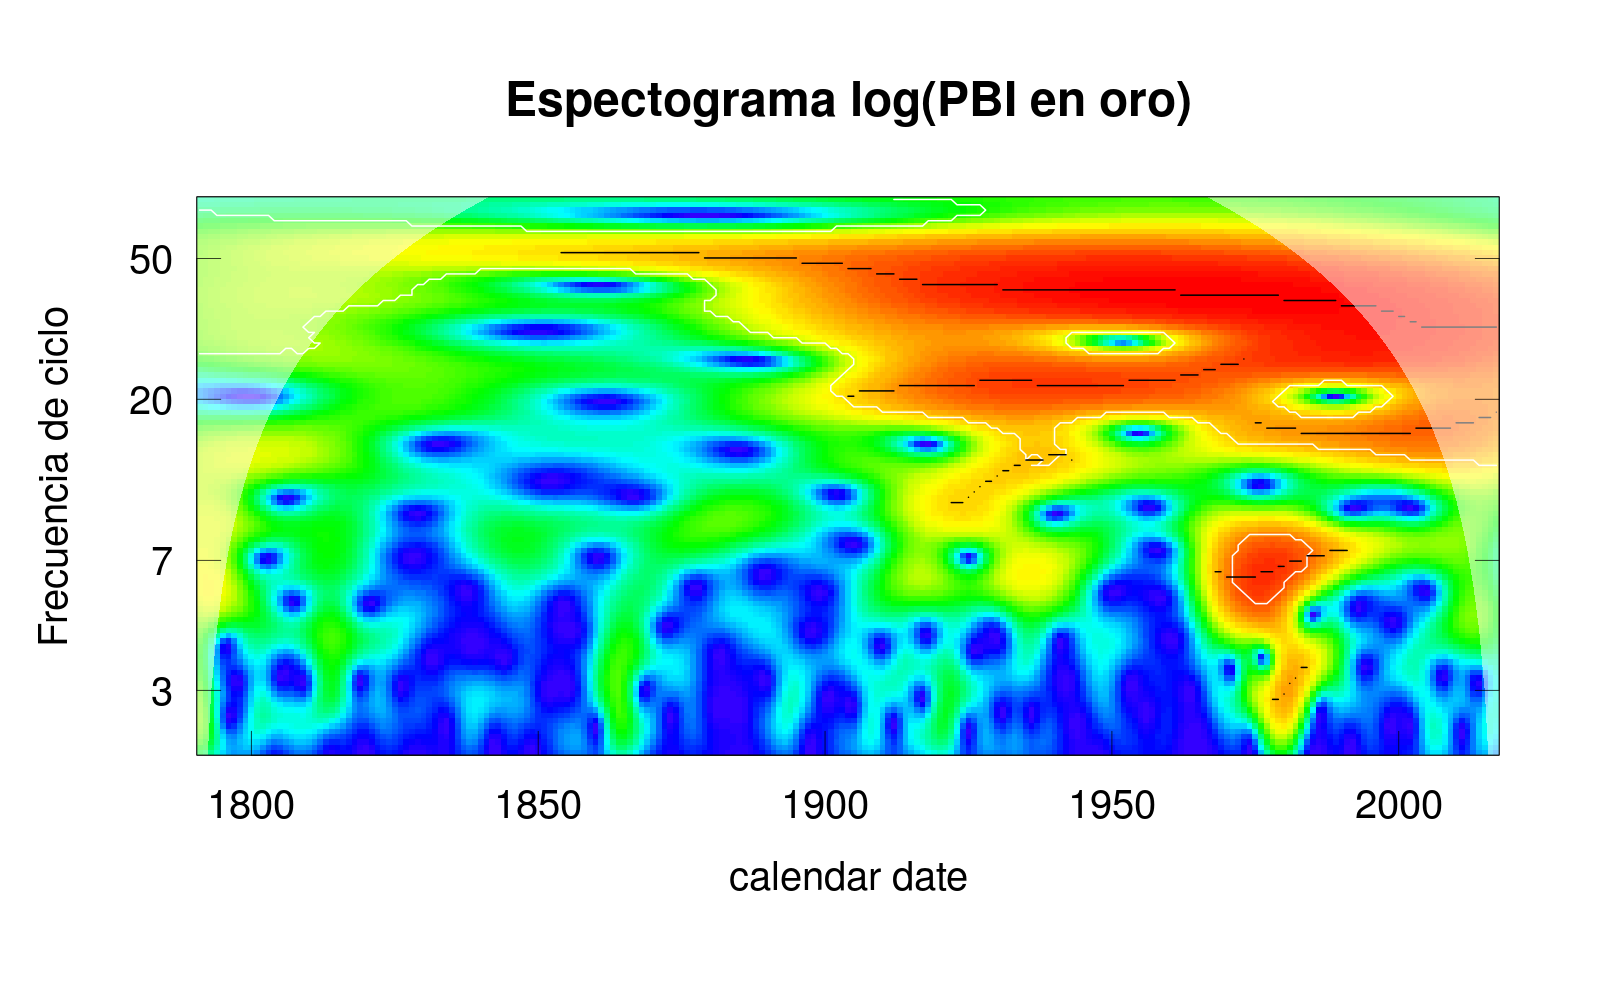
\includegraphics[width=0.75\linewidth]{espectograma_log_gdp.png}
	\label{fig:espect_PBI_b}}
	\caption{Espectograma PBI en oro} \label{fig:espect_PBI}
\end{figure}

las figuras \ref{fig:espect_wg} muestran los espectogramas de la serie del salario expresado en oro \ref{fig:espect_wg_a} y el mismo tomado en logaritmo en \ref{fig:espect_wg_b}. Para esta serie nuevamente se observa un ciclo largo bien definido en torno a los 50 años, especialmente si se observa la serie tomada en base logarítmica. Este ciclo largo parece oscilar entre las frecuencias de $1/32$ y $1/64$, cayendo en el tiempo. Por su parte, se delimita un segundo ciclo, en torno a los 16 años de extensión, y finalmente un ciclo corto de entre 6 y 8 años.  Al tomar la escala logarítmica, también aparece un ciclo de mayor frecuencia, de unos 3 años de duración. En consecuencia, ambas series parecen arrojar resultados en concordancia, sean o no tomadas en logaritmo. 

\begin{figure}[H]
	\centering
	\subfigure[Salario]{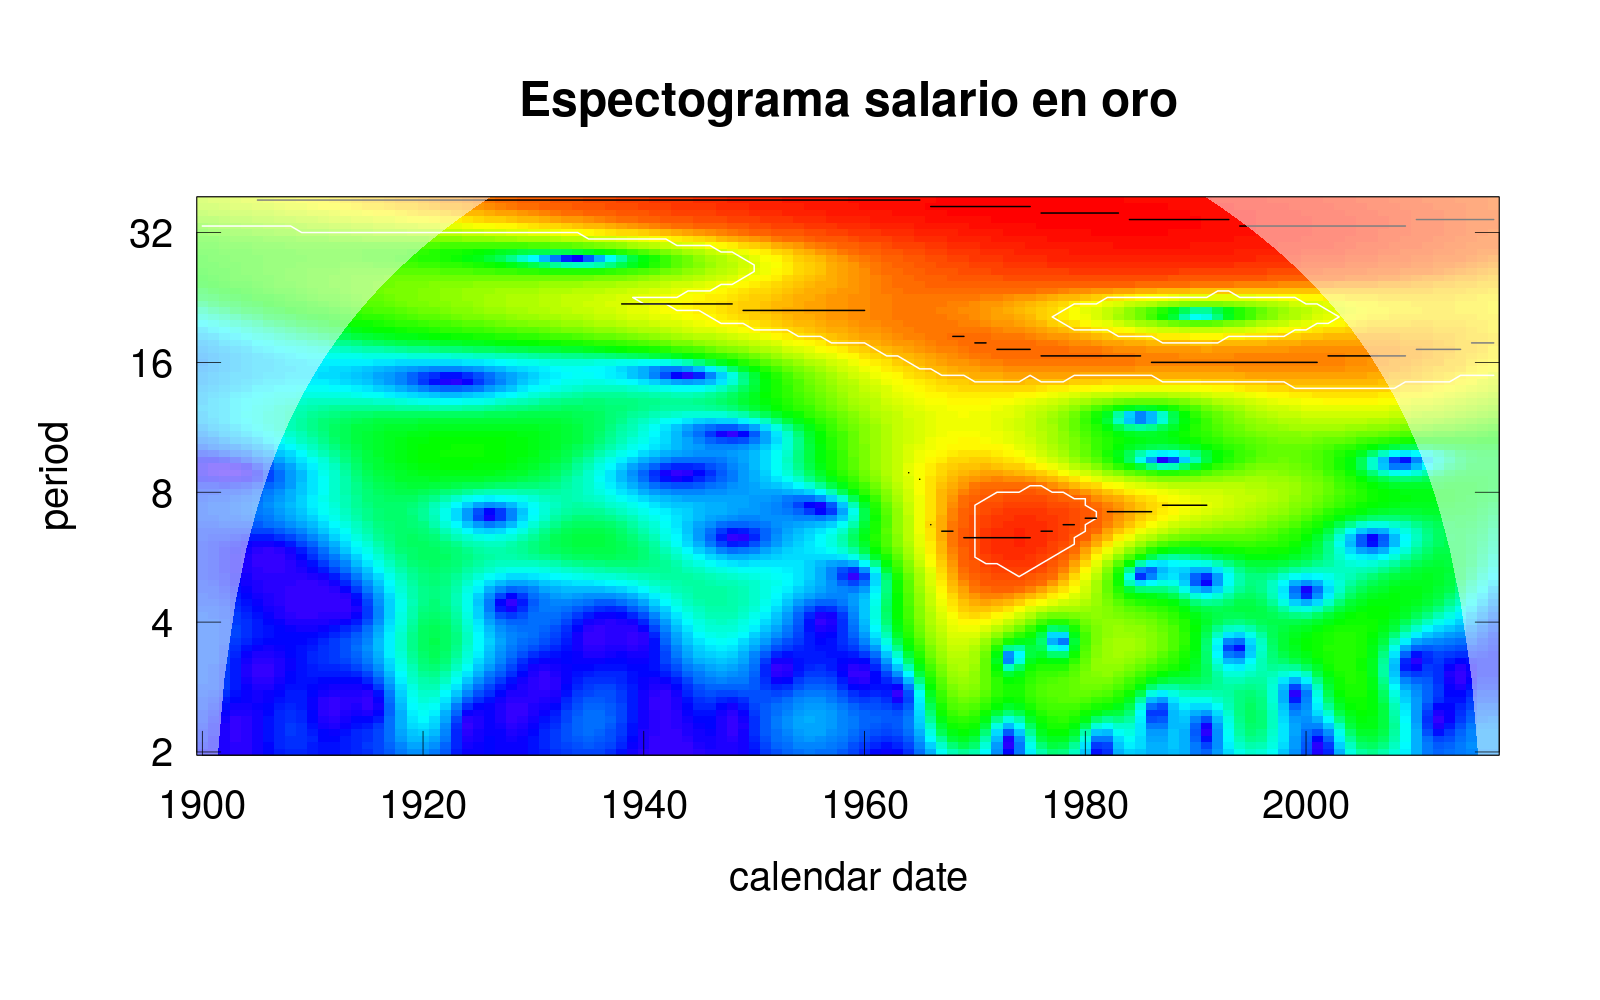
\includegraphics[width=0.75\linewidth]{espectograma_wg.png}
	\label{fig:espect_wg_a}}
	\subfigure[$log(Salario)$]{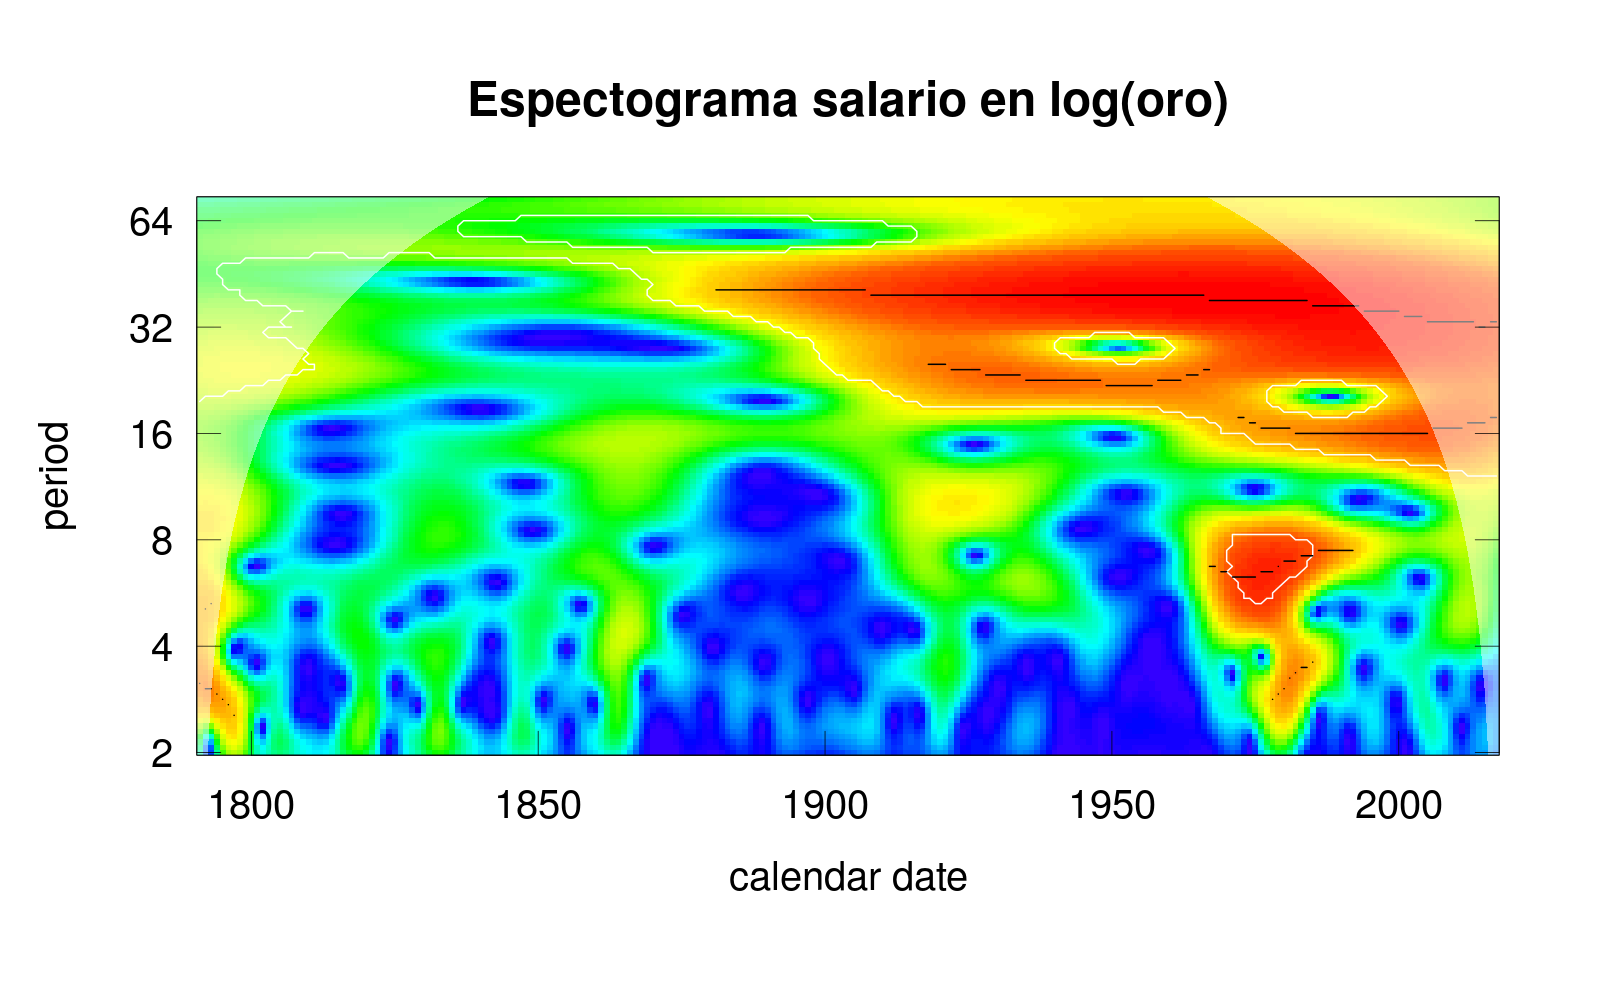
\includegraphics[width=0.75\linewidth]{espectograma_log_wg.png}
	\label{fig:espect_wg_b}}
	\caption{Espectograma Salario en oro} \label{fig:espect_wg}
\end{figure}


En la figura \ref{fig:espect_uk} se muestra la serie del PBI expresado en oro para el Reino Unido entre 1700 y 1900. Al igual que en las series anteriores se expresa la serie sin transformaciones adicionales en \ref{fig:espect_uk_a} y expresada en logaritmo en \ref{fig:espect_uk_b}. A diferencia de la serie de Estados Unidos, aquí se puede observar con más claridad el ciclo corto, en torno a los 10 años. 


\begin{figure}[H]
	\centering
	\subfigure[PBI UK]{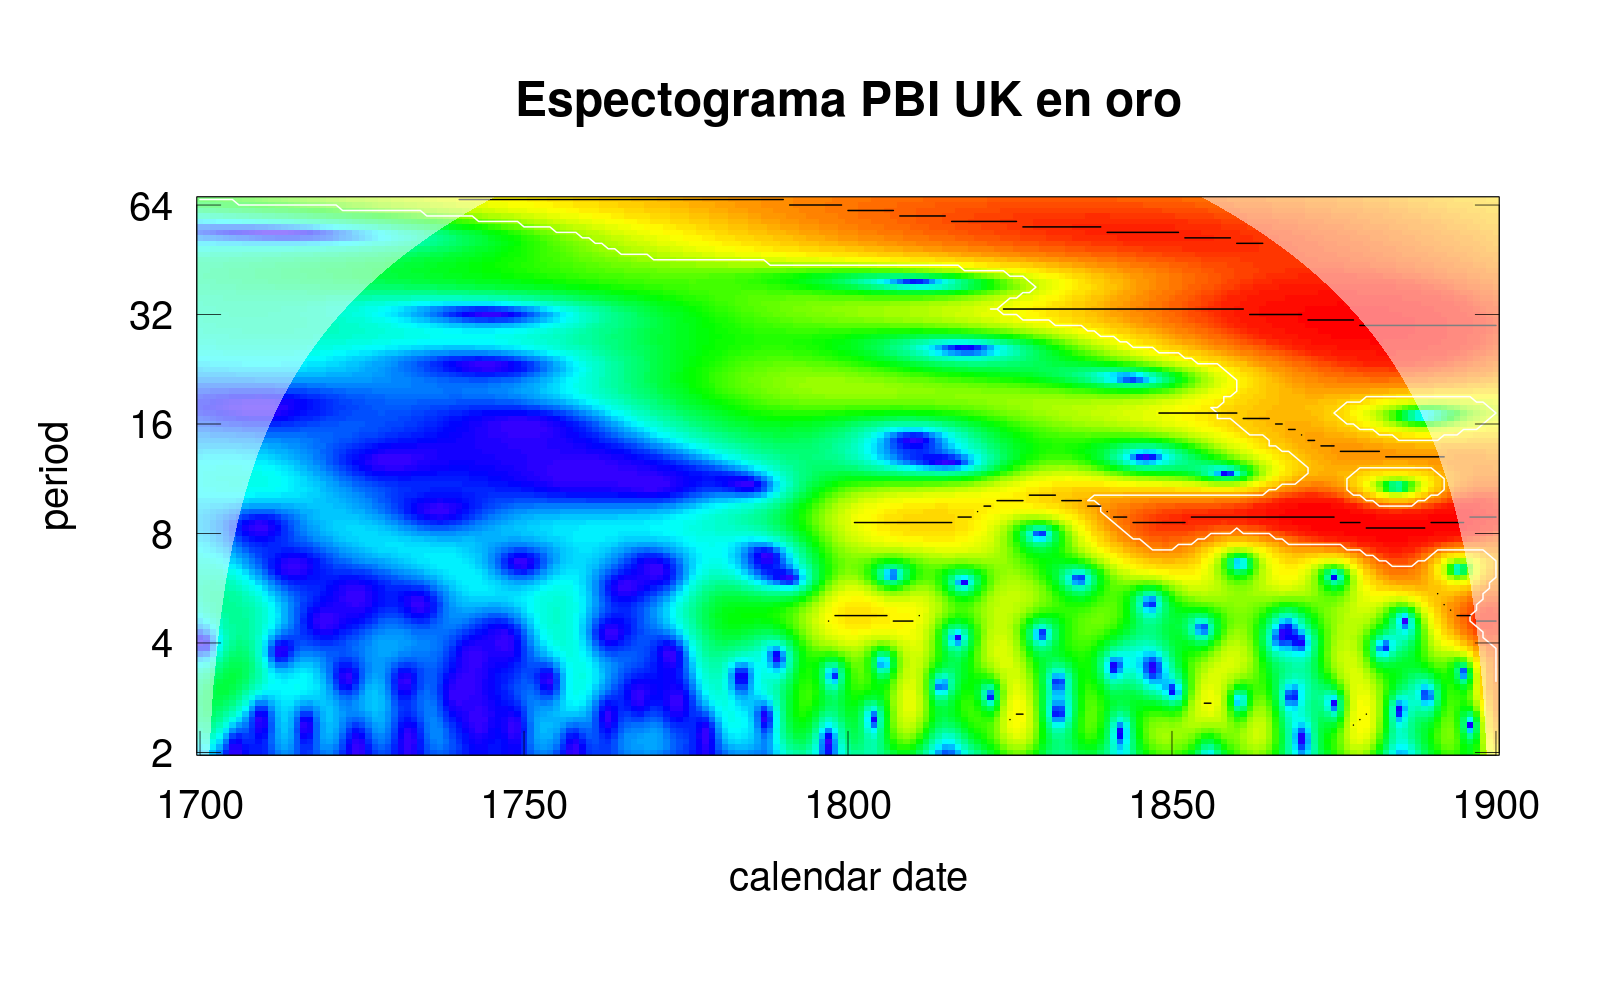
\includegraphics[width=0.75\linewidth]{espectograma_gdp_uk.png}
		\label{fig:espect_uk_a}}
	\subfigure[$log$(PBI UK)]{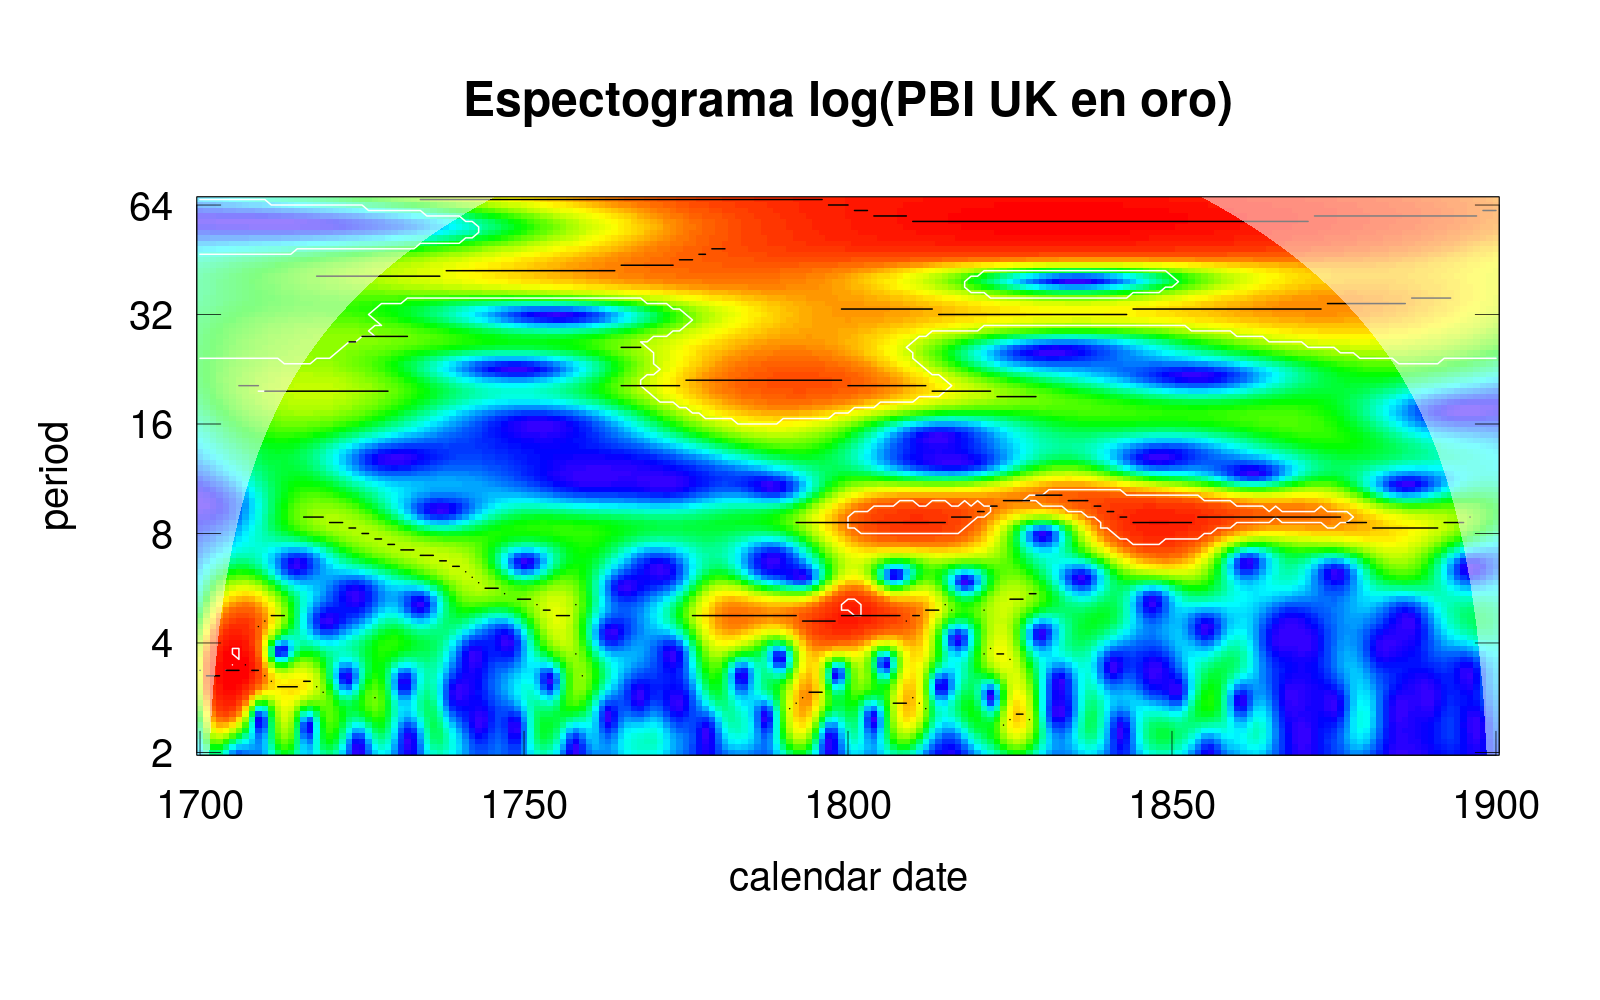
\includegraphics[width=0.75\linewidth]{espectograma_log_gdp_uk.png}
		\label{fig:espect_uk_b}}
	\caption{Espectograma PBI Reino Unido} \label{fig:espect_uk}
\end{figure}

A su vez, otra diferencia que destaca es que en las figuras de Reino Unido el efecto de la transformación logarítmica es mayor que en las series anteriores. De esta forma, en \ref{fig:espect_uk_b} se puede observar una multiplicidad de ciclos que destacan como influyentes. En particular, el más corto pareciera estar en torno a los cuatro años de duración, especialmente presente al principio de la serie y en el entorno del 1800. Luego destaca el ciclo en torno a los 8 años de duración, asociado en la descripción realizada en el Análisis Exploratorio de Datos con lo que se marcaba como un ciclo de 10 años. De mayor extensión temporal se intercala un ciclo en torno a los 20 años, al principio de la serie y en el entorno del 1800, junto con un ciclo de 30-35 años en los períodos restantes. Finalmente, vuelve a registrarse un ciclo largo, en torno a los  64 años de extensión. 

Es importante registrar el efecto que produce la tendencia de la serie sobre los espectogramas. En la figura \ref{fig:uk_gdp} se observaba un fuerte efecto tendencial del producto expresado en oro para el Reino Unido durante los siglos XVIII y XIX. Dicha tendencia no pareciera ser lineal y por lo tanto resulta de interés analizar las posibles distorsiones que esto puede generar sobre los espectogramas. en la figura \ref{fig:tendencias} se puede observar el PBI del Reino Unido en oro, junto con un suavizado lineal mediante un modelo de regresiones locales \citep{Shyu1992}, y la serie resultante de eliminar dicha tendencia. 

En efecto, en la figura \ref{fig:espectograma_gdp_uk_Tend} se observa el espectograma de la tendencia calculada sobre la serie. Allí se destaca el período en torno a los cincuenta años, lo que pareciera indicar que aquello descripto hasta este momento es un simple efecto tendencial oculto en los espectogramas. Sin embargo, en la figura \ref{fig:espectograma_sin_tend} se observa el espectograma de la serie del producto para el Reino Unido, expresado en oro, pero luego de restar la tendencia de la serie. Se puede apreciar que dicho espectograma es casi idéntico al visto anteriormente en la figura \ref{fig:espect_uk_a}. Esto quiere decir que la técnica de wavelets no se ve afectada por la tendencia subyacente de las series analizadas.

\begin{figure}[H]
	\centering
	\subfigure[]{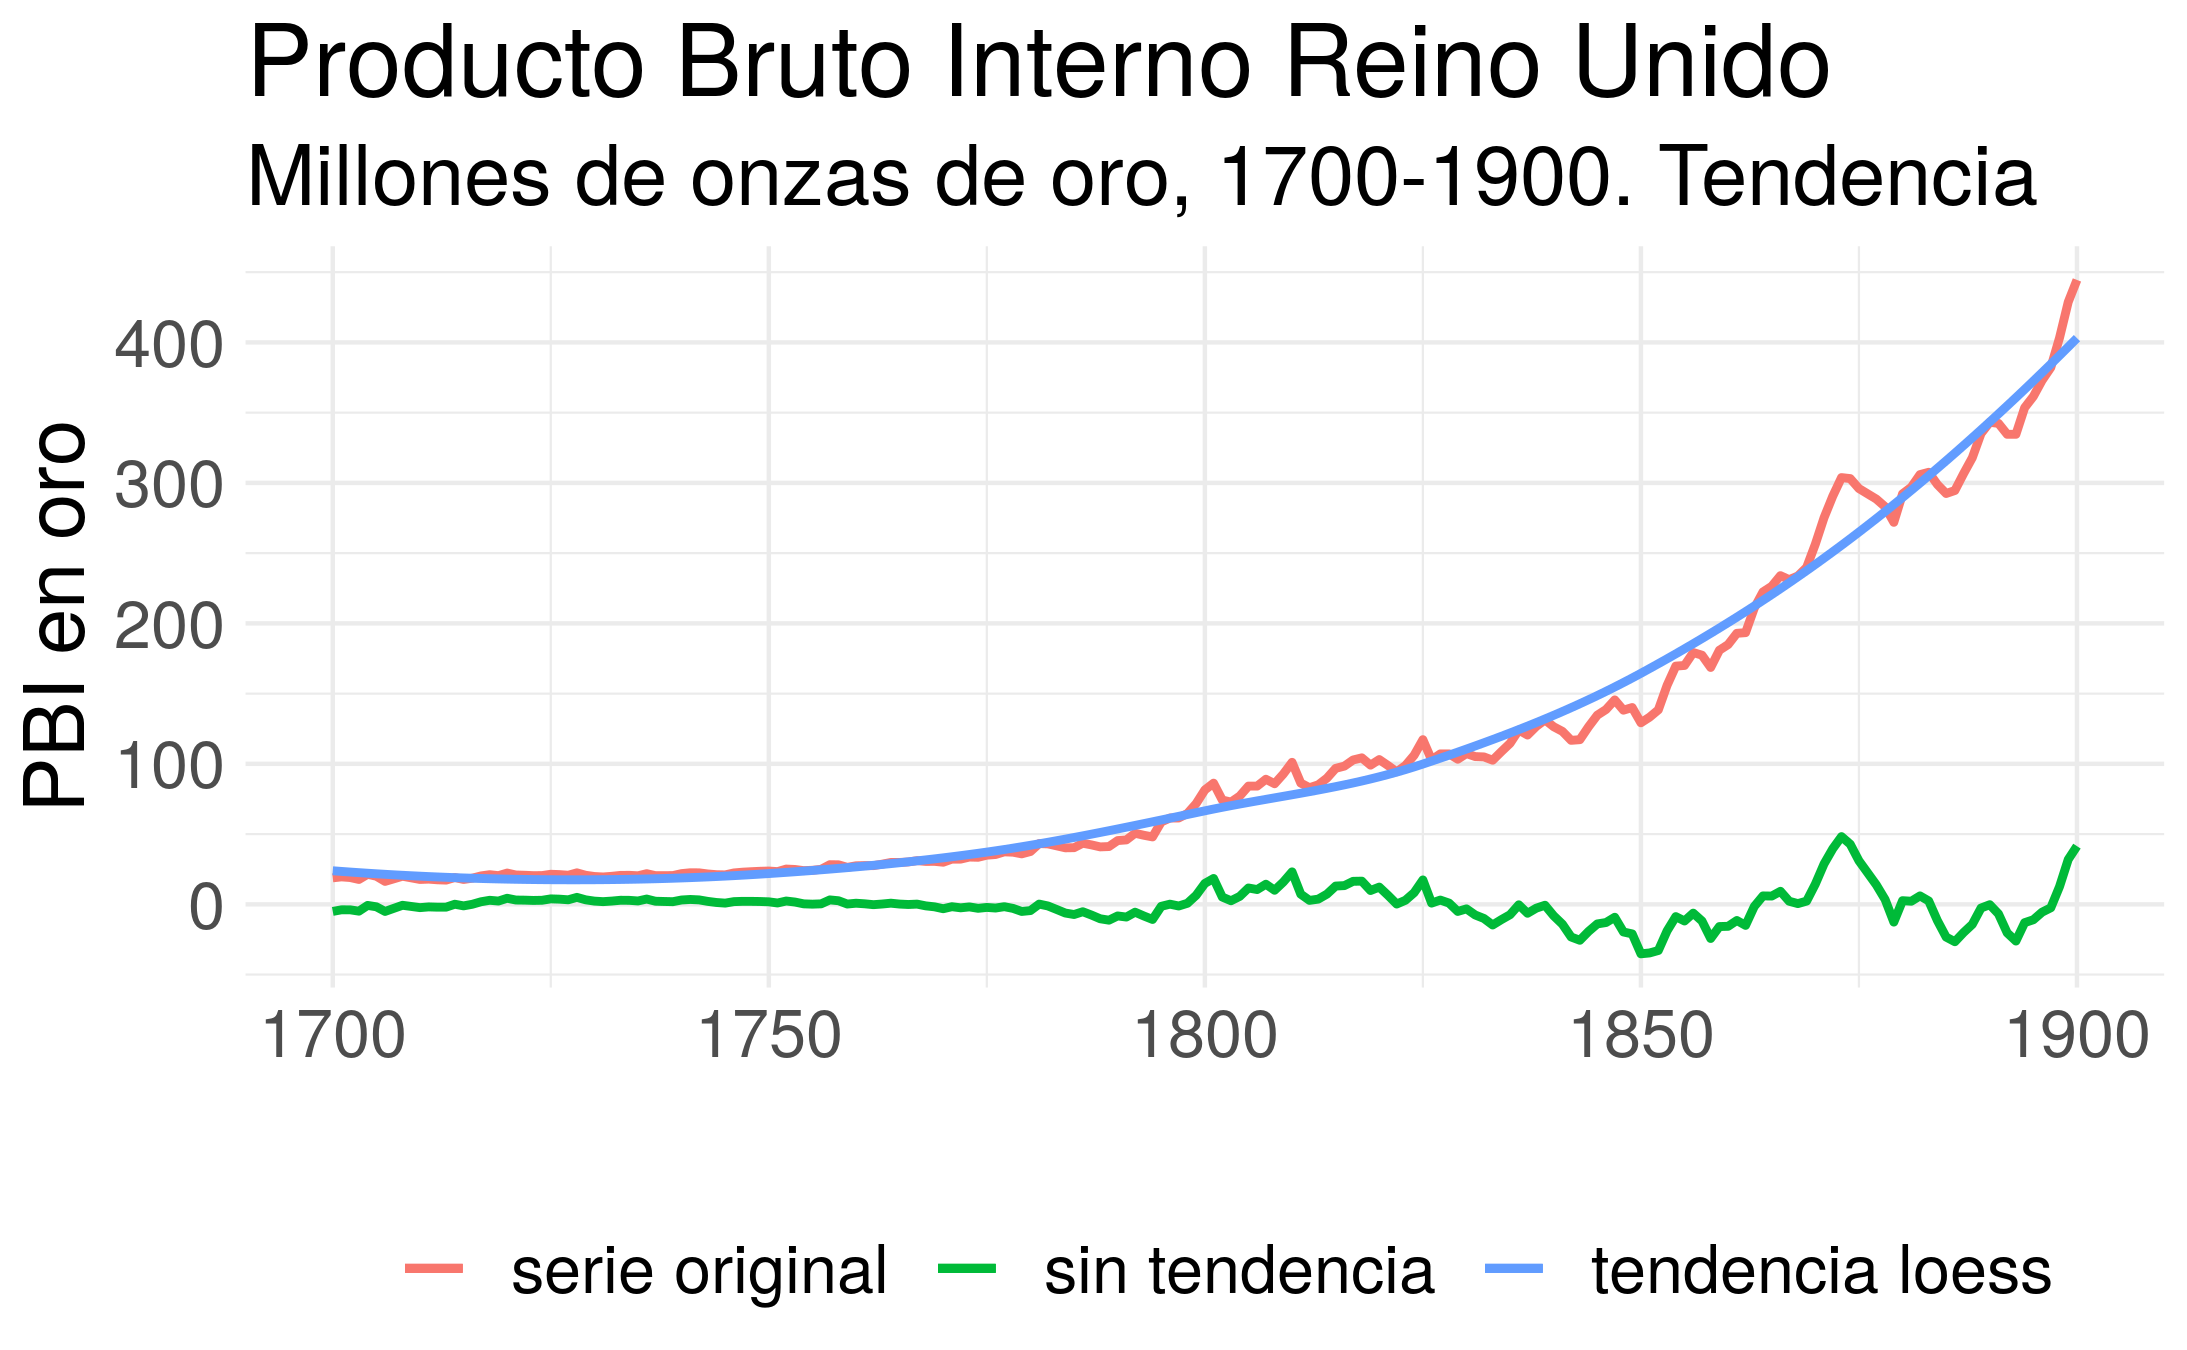
\includegraphics[width=0.75\linewidth]{pbi_uk_tendencias.png}
		\label{fig:tendencias}}
	\subfigure[]{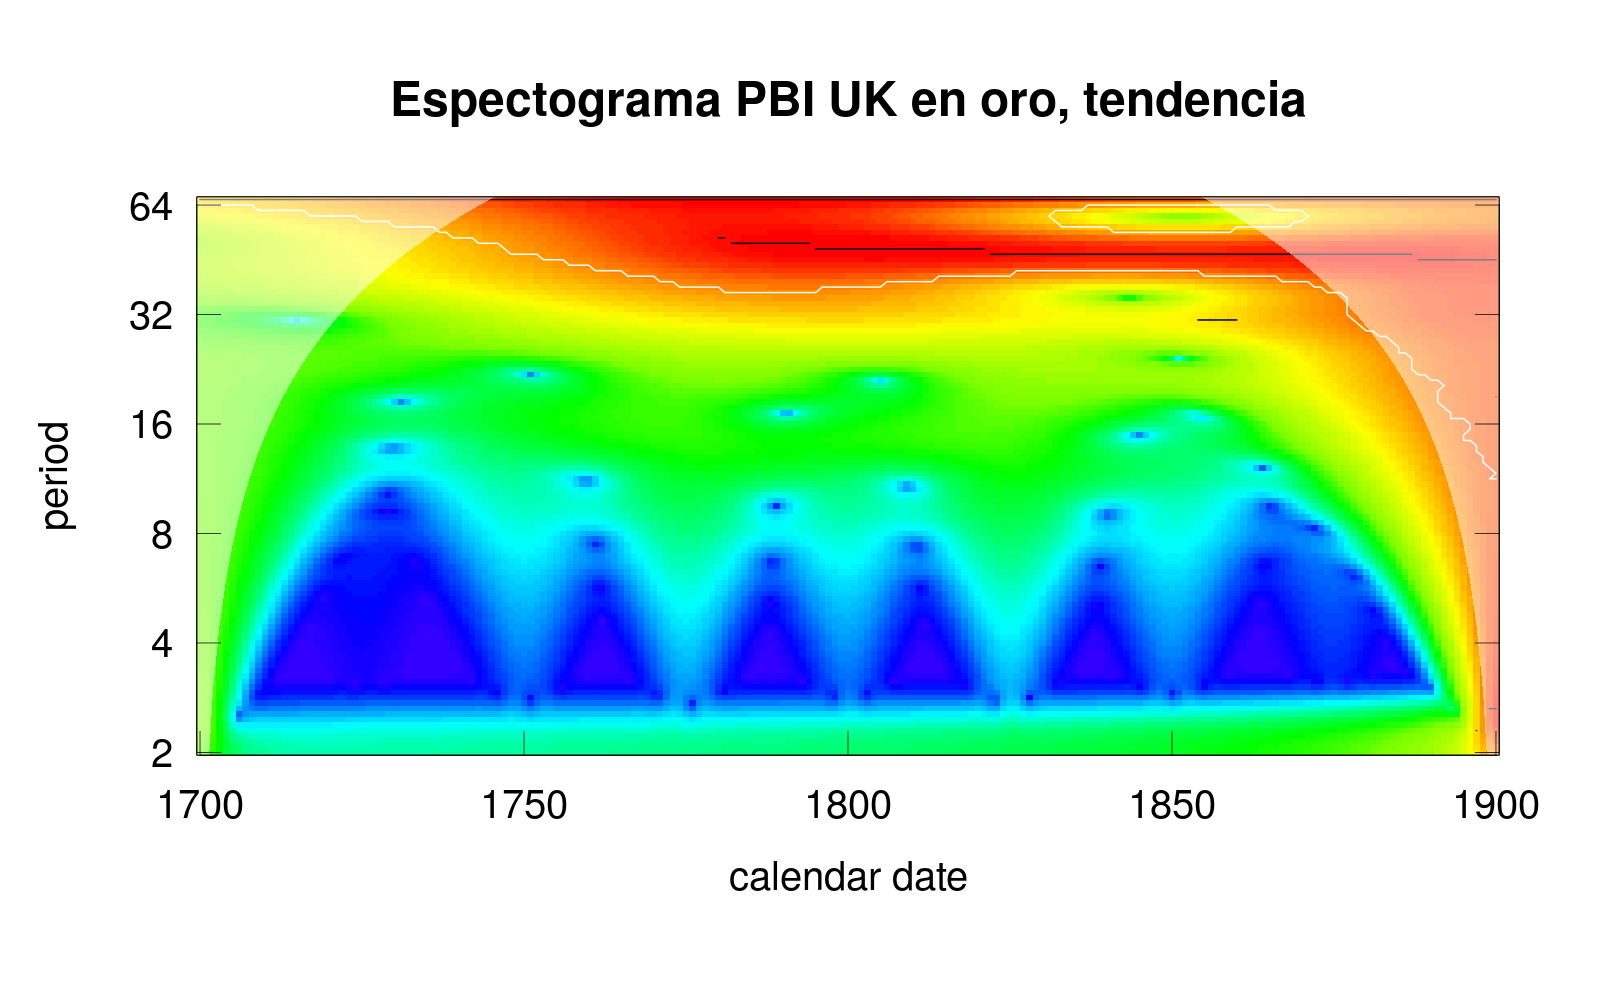
\includegraphics[width=0.48\linewidth]{espectograma_gdp_uk_Tend.png}
		\label{fig:espectograma_gdp_uk_Tend}}
	\subfigure[]{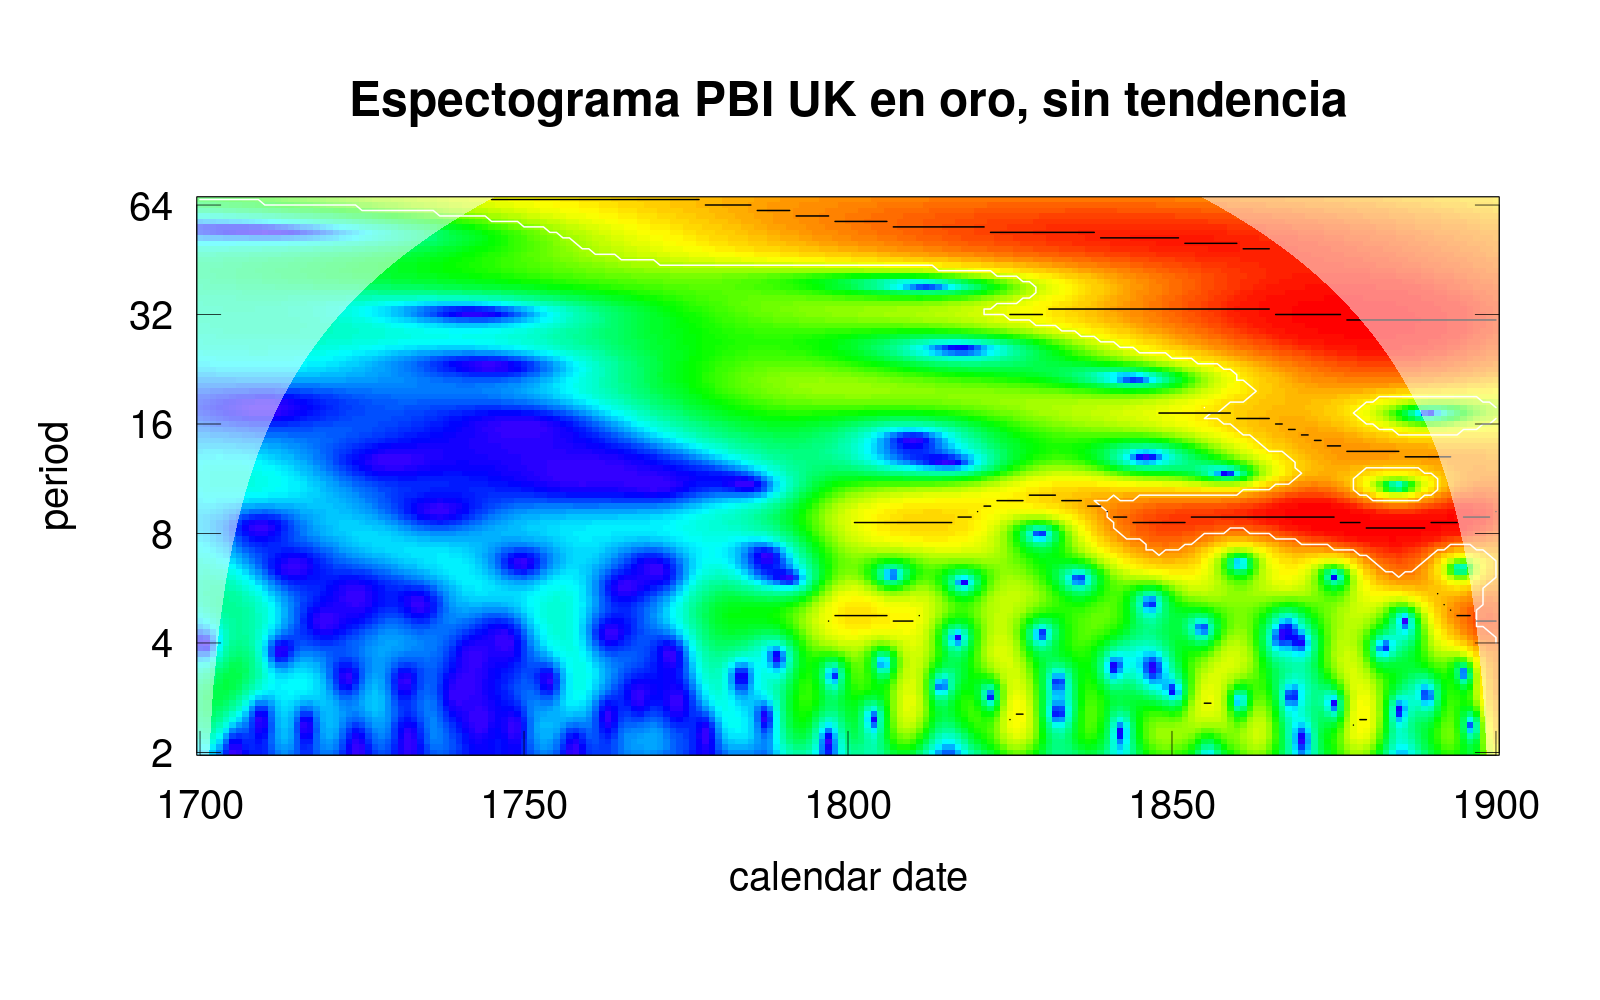
\includegraphics[width=0.48\linewidth]{espectograma_gdp_uk_sinTend.png}
		\label{fig:espectograma_sin_tend}}
	\caption{Efecto tendencia} \label{fig:espect_tendencias}

\end{figure}





\section{Conclusiones}

En el presente trabajo se realizó un recorrido por las principales aproximaciones teóricas respecto al ciclo económico, y se planteó la importancia de un análisis empírico respecto a dicho fenómeno. Para ello, se utilizaron las series de PBI y Salario de Estados Unidos entre 1790 y 2017, expresadas en oro, por los efectos distorsivos que podría generar dicha variable. También se utilizó la serie del PBI para el Reino Unido, entre 1700 y 1900

En el Análisis Exploratorio de Datos se encontró una fuerte correspondencia entre los quiebres de estas series, y las crisis conocidas por la historiografía económica, así como un movimiento oscilatorio aparente que pareciera corresponderse con las ondas largas de Kondratieff para el siglo XX, junto con las particularidades que exhiben las distintas series según el período de tiempo considerado. Por su parte, el siglo XIX en Reino Unido pareciera resaltar las crisis en torno a los 10 años de duración.

Luego se realizó un análisis en base a \textit{Wavelets}, una herramienta poco utilizada en el análisis económico de las series de tiempo, pero con la cual se puede visualizar la correspondencia de las series económicas con los ciclos a diferentes extensiones. Los resultados de esta técnica muestran la existencia de tres ciclos bien definidos a distintas frecuencias, los cuales se corresponden con las hipótesis estudiadas sobre la existencia de un ciclo corto, uno medio y uno largo. También es importante mencionar que esta herramienta pierde resolución en ciclos de períodos muy largos, y que entre las distintas series analizadas existen ciertas diferencias de nivel en los mismos. En este sentido, la herramienta vista no permite definir con exactitud la extensión temporal de cada uno de los ciclos, sino que simplemente demuestra su existencia.

Es importante remarcar que el objetivo del presente trabajo es buscar evidencia empírica respecto de la frecuencia y amplitud del comportamiento cíclico de la economía. Se toma las series de salario y PBI por ser buenos aproximadores de movimiento económico general, pero no son los únicos. A su vez, como las estadísticas tienen una base nacional, el PBI siempre es de un país en particular, así como las estadísticas del salario, debimos decidir tomar un país particular, como expresión de la economía mundial. En este sentido, al ser Estados Unidos la unidad nacional de la economía mundial de mayor envergadura, optamos por este país como representante de la economía mundial. No obstante, si bien la economía estadounidense es un buen reflejo de los movimientos de la economía mundial durante el siglo XX, lo mismo no se sostiene para el siglo XIX, dado que no se había constituido aún como la primera potencia de la economía mundial. En este sentido, es natural que no se expresen las determinaciones generales de la economía, como el ciclo, para dicho siglo, y observemos evidencia sólo a partir del 1900. Es por ello que el análisis de las series estadounidenses se complementó con las series de Reino Unido para los dos siglos precedentes. 

Como conclusión, la utilización de esta técnica para el estudio de series históricas, ampliamente estudiadas por la bibliografía especializada, pareciera ser útil para obtener nueva información de los datos utilizados. Los resultados apuntan a la confirmación de la existencia de series de media y larga duración, si bien la regularidad empírica no es suficiente para determinar con exactitud la frecuencia de dichos ciclos. En otros términos, si bien la intuición de \cite{kuznets1930secular} y \cite{kondratieff1979long} se confirma, los resultados son menos promisorios respecto de la posibilidad de definir con precisión el fenómenos. Incluso más, la evidencia pareciera apuntar a que la frecuencia de los ciclos de media y larga duración podría variar parcialmente a lo largo de la historia. 

El presente trabajo plantea sendas lineas de investigación, especialmente respecto de la utilización de la técnica Wavelets en nuevas series, tanto para series de variables financieras, como series de PBI y salario de otros países.


\bibliography{bibliography.bib}



\end{document}
